\documentclass[A4paper, 12pt, oneside]{book}
\usepackage{socstyle}
\def\asydir{asy}

\begin{document}
%{{{ Úvodní SOČ stránky
\pagestyle{empty}
\topskip0pt
\begin{center}
	{\fontsize{18pt}{22pt}\selectfont \B{\S{Středoškolská odborná činnost}}} \\
	{\fontsize{14pt}{17pt}\selectfont \B{{Obor č. 2: Fyzika}}}
\end{center}
\vfill
\begin{center}
	{\fontsize{20pt}{26pt}\selectfont \B{Mechanika rodin planetek \\[6pt] s~aplikací na rodinu Eunomia}}
\end{center}
\vfill
{\large \bfseries Adam Křivka \\
	Jihomoravský kraj \hfill Brno 2018}
\newpage

\begin{center}
	{\fontsize{18pt}{22pt}\selectfont \B{\S{Středoškolská odborná činnost}}} \\
	{\fontsize{14pt}{17pt}\selectfont \B{{Obor č. 2: Fyzika}}}
\end{center}
\vfill
\begin{center}
	{\fontsize{20pt}{26pt}\selectfont \B{Mechanika rodin planetek \\[6pt] s~aplikací na rodinu Eunomia}}

	 {\fontsize{20pt}{26pt}\selectfont \B{Asteroid families mechanics \\[6pt] with application to the family Eunomia}}
\end{center}
\vfill
\begin{tabularx}{\textwidth}{lX}
	{\bfseries Autoři:} & Adam Křivka \\
	{\bfseries Škola:} & Cyrilometodějské gymnázium a střední odborná škola pedagogická Brno, Lerchova 63, 602 00 Brno \\
	{\bfseries Kraj:} & Jihomoravský kraj \\
	{\bfseries Konzultant:} & doc. Mgr. Miroslav Brož, Ph.\,D.
\end{tabularx}

\

\noindent Brno 2018

\newpage

{\large \bfseries Prohlášení}

Prohlašuji, že jsem svou práci SOČ vypracoval/a samostatně a použil/a jsem pouze prameny a literaturu uvedené v~seznamu bibliografických záznamů.

Prohlašuji, že tištěná verze a elektronická verze soutěžní práce SOČ jsou shodné. 

Nemám závažný důvod proti zpřístupňování této práce v~souladu se zákonem č. 121/2000 Sb., o~právu autorském, o~právech souvisejících s~právem autorským a o~změně některých zákonů (autorský zákon) ve znění pozdějších předpisů. 

\

V~Brně dne \today\ \dotfill \hspace{10mm}

\newpage

{\large \bfseries Poděkování}

\newpage

{\large \bfseries Anotace}

{\large \bfseries Klíčová slova}

{\large \bfseries Annotation}

{\large \bfseries Keywords}

\newpage

\tableofcontents

\newpage %}}}
\pagestyle{headings}
\chapter{Úvod}
Planetky (někdy nepřesně označovány jako asteroidy) jsou nejpočetnější skupinou těles ve sluneční soustavě a svým způsobem také nejpodstatnější a nejzajímavější. První planetka byla objevena v roce 1801 italským matematikem Giuseppem Piazzim (1746--1826) --- touto \uv{planetkou} byl Ceres, který je ale v dnešní době již považován za trpasličí planetu. Dnes je již známo přes půl milionu planetek (konkrétně katalog použitý v této práci cite{broz18}??? obsahuje $524\,138$ vstupů).

Pod pojmem rodina planetek rozumíme skupinu planetek vzniklou rozpadem stejného mateřského tělesa, který byl způsoben srážkou s jiným tělesem. Poprvé si těchto skupin v roce 1918 všiml japonský astronom Kiyotsugu Hirayama (1874--1943), po němž jsou mimo jiné pojmenovány tzv. \uv{Hirayamovy rodiny}, mezi které patří Themis, Koronis a Eos, později také Flora a Maria, naši rodinu Eunomia bohužel Hirayama nezpozoroval. 

Studiem těchto kolizních rodin můžeme zjistit mnoho informací o vzniku sluneční soustavy a její dynamické struktuře. Dále jimi můžeme podpořit teorii o \textit{Velkém pozdním bombardování} (LHB --- \textit{Late Heavy Bombardment}), která říká, že před přibližně $4,1$ až $3,8$ miliardami let došlo migraci planet (Neptun se prohodil s Uranem), která způsobila difuzi těles na okraji sluneční soustavy, která nato začala bombardovat vnitřní sluneční soustavu (viz krátery na Měsíci).

\section{Struktura práce}
V následující (druhé) kapitole této práce vybudujeme nutné matematicko--fyzikální znalosti k pochopení samotného předmětu výzkumu, který je popsán v kapitole čtvrté. Prostřední (třetí) kapitola je věnována obecným informacím o planetkách a rodinách planetek ve sluneční soustavě a k jejímu pochopení není první kapitola potřeba, ačkoliv k porozumění samotného výzkumu je nutné znát kapitoly všechny. V závěru shrnujeme naše počínání včetně zmínění možností zlepšení práce či budoucího výzkumu. Na úplném konci dokumentu se samozřejmě nachází bibliografie a přílohy obsahující vybrané zdrojové kódy.

\chapter{Nebeská mechanika}
Nebeská mechanika se zabývá pohybem těles ve vesmíru a její studium je stěžejní k pochopení různých dějů ve sluneční soustavě --- od vzniku prvních planet po dráhu kosmických sond. Své počátky má v astronomii, kterou se lidé zabývali už v dávných dobách, kdy se snažili vysvětlit pohyb hvězd po obloze. Největší rozvoj této disciplíny však započal až ve středověku, kdy Isaac Newton (1642--1726) v roce 1687 poprvé definoval pohybové zákony a gravitační zákon, na kterých stojí dalo by se říct celá nebeská mechanika. Další významnou událostí byl vzestup počítačů, který umožnil dlouhé simulace sluneční soustavy, čímž bylo zjištěno mnoho nových informací například o formaci planet nebo rodin planetek.

\section{Pohybové rovnice}
Pohybová rovnice je matematicky zapsaný fyzikální vztah, který popisuje možné pohyby těles v~daném prostředí \cite{wiki:eqm}. Řešením pohybové rovnice je funkce, popisující polohu a rychlost každého zkoumaného tělesa v~závislosti na čase. Přitom potřebujeme znát počáteční podmínky --- polohy a rychlosti těles na začátku. Pohybová rovnice bývá ve tvaru diferenciální rovnice, což je rovnice, která vyjadřuje vztah mezi nějakou funkcí a jejími derivacemi\footnote{Derivace označuje okamžitou změnu hodnoty funkce při velmi malé změně argumentu, v~našem případě času.}.

V~následující části se pokusíme nalézt řešení pohybové rovnice pro tělesa ve sluneční soustavě. Zákony, jimiž se budou naše tělesa řídit, jsou již zmíněné Newtonovy pohybové zákony a Newtonův gravitační zákon.
\subsection{Rovnice pro dvě tělesa} \label{sec:2body}
Omezme se nyní na dvě tělesa a nalezněme řešení tzv.\ problému dvou těles --- Keplerovy úlohy. To znamená, že se pokusíme odvodit funkci, popisující polohu a rychlost obou těles v~závislosti na čase. 

Nacházíme se v~inerciální vztažné soustavě, což je taková vztažná soustava, kde platí první Newtonův zákon. Jako bod v~klidu si zvolme těžiště soustavy. Pro síly působící na obě tělesa podle Newtonova gravitačního zákona a druhého a třetího pohybového zákona platí
\begin{align} 
	\vec{F}_1 &= +G\frac{m_1m_2}{\abs{\vec{r}}^3}\vec{r} = m_1\vec{a}_1\,, \label{eq:newton1} \\
	\vec{F}_2 &= -G\frac{m_1m_2}{\abs{\vec{r}}^3}\vec{r} = m_2\vec{a}_2\,, \label{eq:newton2}
\end{align}
kde $G$ označuje gravitační konstantu, $m_1$, $m_2$ hmotnosti zkoumaných těles, $\vec{a}_1$, $\vec{a}_2$ vektory\footnote{Připomeňme, že vektor je veličina, která velikost i směr. Je určen souřadnicemi, které jsou v této práci podle kontextu dvourozměrné $x,\,y$ nebo trojrozměrné $x,\,y,\,z$.}  zrychlení těles (tj.\ druhé derivace polohových vektorů $\vec{r}_1$, $\vec{r}_2$ podle času) a $\vec{r}$ vektor udávající vzájemnou polohu těles, definovanou jako $\vec{r} \equiv \vec{r}_2 - \vec{r}_1$. Sečtením obou rovnic dostáváme
\begin{align} \label{eq:mr0}
	\vec{F}_1 + \vec{F}_2 = m_1\vec{a_1} + m_2\vec{a_2} = \vec{0}\,.
\end{align}
Vektor popisující polohu těžiště soustavy je $\vec{R} \equiv \frac{m_1\vec{r}_1 + m_2\vec{r}_2}{m_1 + m_2}$. Jeho druhou derivací podle času dostáváme zrychlení
\begin{align}
	\diff[2]{\vec{R}}{t} = \frac{m_1\vec{a_1} + m_2\vec{a_2}}{m_1+m_2} = \vec{0}\,,
\end{align}
které se podle \eqref{eq:mr0} rovná nule, takže se těžiště soustavy pohybuje konstantní rychlostí.

Nyní se však přesuňme do soustavy neinerciální, kde je první z~těles (běžně to hmotnější) nehybné. Označme $\vec{a}\equiv\vec{a}_2-\vec{a}_1$ zrychlení druhého tělesa vzhledem k~prvnímu. Po pokrácení $m_1$ a $m_2$ můžeme odečíst upravenou rovnici~\eqref{eq:newton1} od upravené rovnice~\eqref{eq:newton2}, čímž dostaneme
\begin{align}
	\nonumber \vec{a}_2 - \vec{a}_1 = -Gm_1\frac{\vec{r}}{\abs{\vec{r}}^3}-Gm_2\frac{\vec{r}}{\abs{\vec{r}}^3}\,, \\
	\nonumber \vec{a} = -G(m_1+m_2)\frac{\vec{r}}{\abs{\vec{r}}^3}\,, \\
		\diff[2]{\vec{r}}{t} + G(m_1+m_2)\frac{\vec{r}}{\abs{\vec{r}}^3} = \vec{0}\,. \label{eq:eqmotion}
\end{align}
Často ještě definujeme gravitační parametr soustavy $\mu\equiv G(m_1+m_2)$.

I~přesto, že tato diferenciální rovnice ještě není ve své konečné podobě vhodné k~tomu, abychom z~ní odvodili následující vztah, prozradíme, že je jím funkce v~polárních souřadnicích, popisující vzdálenost těles $r\equiv\abs{\vec{r}}$ v~závislosti na \I{pravé délce} $\theta$, což je úhel, který svírá přímka procházející oběma tělesy a nějaká zvolená referenční přímka, přesné odvození viz~\cite{murray00}.
\begin{align} \label{eq:polar}
	r(\theta)=\frac{p}{1+e\cos{(\theta-\omega)}}\,.
\end{align}
Vztah \eqref{eq:polar} je obecným předpisem kuželosečky --- hyperboly, paraboly, elipsy nebo kružnice; pro naše účely se zaměřme na případ elipsy, kdy se v~jednom z~jejích ohnisek nachází centrální těleso.

Veličina $p$ označuje \I{parametr elipsy}, jehož velikost je určena hodnotou $\mu$ a veličinou~$h=|\vec{h}| \equiv \vec{r}\times\diff{\vec{r}}{t}={\rm konst.}$\footnote{což je \uv{něco jako} moment hybnosti systému na jednotku hmotnosti $\mu$. Vycházíme z~předpokladu, že síly působící mezi tělesy (né nutně splňující Newtonův gravitační zákon) jsou stejně velké a působí proti sobě, tedy $\vec{r}\times\vec{a}=\vec{r}\times\diff[2]{\vec{r}}{t}=0$, z~čehož integrací vzhledem k~času můžeme vyvodit právě $\vec{r}\times\diff{\vec{r}}{t}=\vec{h}$, kde $\vec{h}$ je vektor kolmý na rovinu obíhání těles.}, kde $\times$ značí vektorový součin, jako
\begin{align}
	p=\frac{h^2}{\mu}\,,
\end{align}
a pro který dále platí geometrický vztah
\begin{align}
	p=\frac{b^2}{a}\,,
\end{align}
kde $a$ označuje délku hlavní poloosy, což je úsečka spojující střed elipsy s~jedním z~průsečíků elipsy s~hlavní osou --- přímkou spojující ohniska, a $b$ délku vedlejší poloosy, což je úsečka spojující střed elipsy s~průsečíkem elipsy s~přímkou kolmou na hlavní poloosu a procházející středem elipsy --- vedlejší osou (viz obrázek~\ref{fig:elip}).

\begin{figure}
	\centering
	\asyinclude{asy/elip.asy}
	\caption{Eliptická oběžná dráha vesmírného tělesa. Veličina $a$ označuje délku hlavní poloosy, $b$ délku vedlejší poloosy, $\omega$ argument pericentra, $C$ střed elipsy, $F_1$ a $F_2$ polohy ohnisek elipsy, přičemž centrální těleso se nachází v~bodě $F_1$ a pericentrum, resp.\ apocentrum označují body nejmenší, resp.\ největší vzdálenosti od centrálního tělesa.} \label{fig:elip}
\end{figure}

Dále $e$, resp.\ $\omega$ jsou integrační konstanty a nazývají se \I{excentricita} (česky \I{výstřednost}), resp.\ \I{argument pericentra}. Pro excentricitu platí vztah
\begin{align}
	e=\sqrt{1-\frac{b^2}{a^2}}\,,
\end{align}
a volně řečeno udává, jak moc se elipsa liší od kružnice. Hodnota excentricity se pro eliptické dráhy nachází v~intervalu $(0,\,1)$, kde krajními případy jsou $e=0$: dráha má tvar kružnice, a $e=1$: dráha má tvar úsečky.

Argument pericentra $\omega$ je úhel, který svírá hlavní osa s~referenční přímkou. Platí pro něj vztah
\begin{align}
	\theta=\omega+f\,,
\end{align}
kde $f$ označuje \I{pravou anomálii}, což je úhel, který svírá hlavní osa s~průvodičem tělesa (viz obrázek~\ref{fig:E}).

\begin{figure}[!htb] 
	\centering
	\asyinclude{asy/Ef.asy}
	\caption{Ilustrace vztahu mezi excentrickou anomálií $E$ a pravou anomálií $f$. Veličiny $a$, resp.\ $b$ značí délku hlavní, resp.\ vedlejší poloosy, $P$ značí polohu tělesa na elipse, $P'$ průsečík $P$ na kružnici opsanou, $C$ střed elipsy a $F_1,\,F_2$ ohniska elipsy} \label{fig:E}
\end{figure}

Uvědomme si, že jsme neodvodili závislost polohy tělesa na čase. Tuto závislost určuje Keplerova rovnice
\begin{align} \label{eq:kepler}
M = E + e\sin E\,,
\end{align}
kde $M$ označuje \I{střední anomálii}, $E$ \I{excentrickou anomálii} (viz obrázek~\ref{fig:E}) a $e$ excentricitu elipsy. Pro excentrickou anomálii $E$ a pravou anomálií $f$ platí vztah
\begin{align} \label {eq:fE}
	\tan \frac{f}{2} = \sqrt{\frac{1+e}{1-e}}\tan \frac{E}{2}.
\end{align}

Anomálie mají úhlové jednotky, úhel $M$ ale nemůžeme zkonstruovat, nicméně je významný tím, že je lineárně závislý na čase, neboť je určen vztahem 
\begin{align} \label{eq:M}
	M=nt\,,
\end{align}
kde $n$ označuje \I{střední pohyb}, jinak řečeno průměrnou úhlovou rychlost\footnote{ve středoškolském prostředí obvykle značenou jako $\omega$}, pro kterou platí
\begin{align} \label{eq:n}
	n=\frac{2\pi}{T}=\sqrt{\frac{\mu}{a^3}}=\sqrt{\frac{G(m_1+m_2)}{a^3}}\,,
\end{align}
kde $T$ označuje \I{dobu oběhu}. Tento vztah lze lehce odvodit z~Třetího Keplerova zákona, viz~\ref{sec:kepzak}.

Pokud známe excentrickou anomálii $E$, můžeme pomocí Keplerovy rovnice snadno spočítat střední anomálii $M$. Problém spočívá v~tom, že Keplerova rovnice je transcendentní, tedy nemůžeme vyjádřit $E$ v~závislosti na $M$ konečným výrazem, ale pouze nekonečnou řadou nebo jej můžeme aproximovat iteračními nebo numerickými metodami. Řešení Keplerovy rovnice pomocí iterační metody lze nalézt v~příloze~\ref{app:kepit}.

\subsubsection{Keplerovy zákony} \label{sec:kepzak}

Nemůžeme opomenout Keplerovy zákony, které empiricky dokázal Johannes Kepler (1571--1630) a z pohybových rovnic odvodil Newton (1687). Jejich úplné znění, dle~\cite{wiki:kepzak}, je 
\begin{enumerate}[wide]
	\item[\textbf{1. Keplerův zákon}] \ 

Planety obíhají kolem Slunce po eliptických drahách, v~jejichž jednom společném ohnisku je Slunce.
	\item[\textbf{2. Keplerův zákon}] \ 

Obsahy ploch opsaných průvodičem planety (tj.\ spojnice planety a Slunce) za stejný čas jsou stejně velké.
	\item[\textbf{3. Keplerův zákon}] \ 

Poměr druhých mocnin oběžných dob dvou planet je stejný jako poměr třetích mocnin jejich hlavních poloos.
\end{enumerate}

Odvoďme třetí z~těchto zákonů, neboť tím dokážeme vztah~\eqref{eq:n}. Pro jednoduchost se omezme na kruhové oběžné dráhy a situaci, kdy je $m_1 \gg m_2$. Krom Newtonova gravitačního zákona budeme ještě potřebovat vztah pro dostředivou sílu, potřebnou pro obíhání po kružnici
\begin{align}
	F_{\rm d}=\frac{m_2v^2}{r}\,,
\end{align}
kde $v$ označuje rychlost vzhledem k~centrálnímu tělesu, $r$ vzdálenost od centrálního tělesa (v~případě kruhových drah tedy $r=a$, kde $a$ označuje hlavní poloosu) a $m_2$ hmotnost obíhajícího tělesa. Protože dostředivá síla se zde rovná síle gravitační, platí
\begin{align}
	\frac{m_2v^2}{r}&=G\frac{m_1m_2}{r^2}\,,
\end{align}
	odkud
\begin{align}
	v^2&=\frac{Gm_1}{r}\,, \label{eq:dosgrav}
\end{align}
kde $m_1$ označuje hmotnost centrálního tělesa. Dále platí vztah mezi úhlovou a obvodovou rychlostí $v=\omega r$, který můžeme z definice $\omega=\frac{2\pi}{T}$ (podle označení v rovnici~\eqref{eq:n} platí $\omega=n$) dále upravit jako
\begin{align}
	v=\frac{2\pi r}{T}\,,
\end{align}
odkud vyjádříme $T$ a dosadíme~\eqref{eq:dosgrav}, čímž dostaneme
\begin{align}
	T&=\frac{2\pi r}{\sqrt{\frac{Gm_1}{r}}}\,,
\end{align}
	neboli
\begin{align}
	T^2&=\frac{4\pi^2 r^3}{Gm_1}\,.
\end{align}
Dosazením $r=a$ a menší úpravou dostáváme
\begin{align}
	\frac{T^2}{a^3}=\frac{4\pi^2}{Gm_1}={\rm konst.}\,,
\end{align}
což je přibližný tvar třetího Keplerova zákona; poměr $T^2/a^3$ je určen pouze konstantami $\pi$ a $G$ a hmotností centrálního tělesa, je tedy pro všechna tělesa obíhající stejné centrální těleso stejně velký. Pokud bychom vyšli z přesné pohybové rovnice~\eqref{eq:eqmotion}, obdrželi bychom ve jmenovateli $G(m_1+m_2)$. 

\subsection{Rovnice pro N těles}
Jak vidíme, už i pro dvě tělesa se musíme k~získání polohy tělesa v~čase uchýlit k~numerickým metodám. Ukazuje se, že obecný problém $N$ těles je analyticky neřešitelný\footnote{Existují ale zajímavá speciální řešení, viz \cite{cohan12}.} a jediné aplikovatelné metody jsou metody přibližné analytické nebo numerické.

Uvažujme nyní $N$ těles --- respektive hmotných bodů, které na sebe vzájemně gravitačně působí v~souladu s~Newtonovým gravitačním zákonem. Pro libovolné těleso, označené indexem $i\in\{1,\,2,\,\dots,\,N\}$, je celková síla $F_i$, která na něj působí, výslednicí všech gravitačních sil způsobených ostatními tělesy, jak ukazují následující rovnice
\begin{align} 
	\vec{F}_i = m_i\vec{a}_i &= -\sum_{\substack{j=1 \\ j\neq i}}^N G\frac{m_im_j}{\abs{\vec{r}_i-\vec{r}_j}^3}(\vec{r_i}-\vec{r_j})\,, \label{eq:nbody1} \\
		\vec{a}_i &= -\sum_{\substack{j=1 \\ j\neq i}}^N \frac{Gm_j}{\abs{\vec{r}_i-\vec{r}_j}^3}(\vec{r_i}-\vec{r_j})\,, \qquad{\rm pro}\ i\in\{1,\,2,\,\dots,\,N\} \label{eq:nbody2}
\end{align}
kde $\vec{r}_i-\vec{r}_j$ označuje vektor určující vzájemnou polohu těles $i$ a $j$, konkrétně jde o~vektor s~počátkem v~tělese $j$ a koncem v~tělese $i$; ostatní veličiny jsou definované analogicky jako v~předchozí části. Dostáváme tedy soustavu $N$ diferenciálních rovnic ve tvaru~\eqref{eq:nbody2}, kterou vyřešíme numericky.
\subsubsection{Eulerova metoda}\label{sec:euler}
I~přesto, že se následující integrační metoda v~přesných numerických výpočtech zřídka používá, uvádíme ji zde z~didaktických důvodů, neboť názorně ilustruje použití numerických metod pro řešení problému $N$ těles. Jak název napovídá, poprvé s~ní v~18.\ století přišel švýcarský matematik Leonhard Euler (1707--1783).

Princip algoritmu spočívá v~tom, že v~libovolném čase $t$ můžeme z~\eqref{eq:nbody2} vypočítat zrychlení každého tělesa. Pak, po zvolení určitého časového kroku $h$, odpovídajícím způsobem změníme vektor rychlosti. Následně necháme všechna tělesa po dobu časového kroku pohybovat se po přímce konstantní rychlostí. Existují dvě verze Eulerovy metody, dopředná a zpětná, které se liší volbou rychlosti, se kterou necháváme tělesa pohybovat se po přímce, viz následující přesný popis obou metod a obrázek~\ref{fig:euler}.

Mějme zmiňovaných $N$ hmotných bodů, pro které platí~\eqref{eq:nbody2}. Zaměřme se na jeden z~nich a označme jeho počáteční polohu $\vec{r}(t_0)\equiv\vec{r}_0$ a počáteční rychlost $\vec{v}(t_0)\equiv\vec{v}_0$. K~použití Eulerovy metody potřebujeme znát i počáteční polohy a rychlosti všech ostatních těles v~systému. Dále vhodně zvolme velikost časového kroku $h$. V~následujících třech krocích si ukážeme jednu iteraci algoritmu jak pro dopřednou, tak pro zpětnou metodu.

\begin{figure} 
	\centering 
	\begin{subfigure}[b]{0.45\textwidth}
	\asyinclude{asy/f_euler.asy}
	\end{subfigure}
	\begin{subfigure}[b]{0.45\textwidth}
	\asyinclude{asy/b_euler.asy}
	\end{subfigure}
	\caption{Ilustrace dopředné (vlevo) a zpětné (vpravo) Eulerovy metody pro dvě tělesa, kdy větší těleso (velká tečka vlevo nahoře) gravitačně působí na menší těleso (malé tečky vpravo). Jsou ukázány první tři iterace. Algoritmus byl doopravdy implementován, s~počátečními hodnotami: $h=20\,{\rm \text{dnů}}$, $m_1=2\cdot10^{30}\,{\rm kg}$, $G=6,67\cdot10^{-11}\,{\rm m^3\,kg^{-1}\,s^{-2}}$, $|\vec{r}_0|=1\,{\rm AU}$, $v_0=29\,861\,{\rm m\,s^{-1}}$. Vektory jsou vhodně škálované. Šedá křivka znázorňuje analytické řešení problému dvou těles. K nakreslení obrázku byl použit programovací jazyk \I{Asymptote}, viz příloha~\ref{app:asy}.} \label{fig:euler}
\end{figure}
\pagebreak
\begin{enumerate}
	\item Nechť je v~čase $t_k$ poloha zvoleného bodu $\vec{r}(t_k)$ a rychlost $\vec{v}(t_k)$. Z~\eqref{eq:nbody2} vypočítáme zrychlení $\vec{a}(t_k)$. 
	\item Položme $t_{k+1} = t_{k}+h$ a vypočítejme $\vec{v}(t_{k+1}) = \vec{v}(t_k) + h\,\vec{a}(t_k)$.\footnote{Můžeme porovnat se vzorcem pro rovnoměrný přímočarý pohyb, dobře známým ze středoškolského učiva: $v = v_0 + at$, podobně v~kroku $3$: $s = s_0 + vt$.}
	\item Pro dopřednou metodu počítejme $\vec{r}(t_{k+1})$ jako $\vec{r}(t_{k+1}) = \vec{r}(t_k) + h\,\vec{v}(t_k)$ a pro zpětnou jako $\vec{r}(t_{k+1}) = \vec{r}(t_k) + h\,\vec{v}(t_{k+1})$. Poté se vraťme ke kroku $1$, tentokrát počítaje v~čase~$t_{k+1}$. 
\end{enumerate}

Jak můžeme vidět na obrázku~\ref{fig:euler}, vypočtená dráha se od té analytické značně vzdaluje. To by samozřejmě řešila volba menší kroku $h$, ale pro velký počet těles $N$ a velký počet kroků je algoritmus příliš pomalý.

Jedno z~možných vylepšení je volně řečeno průměrování dopředné a zpětné Eulerovy metody --- \uv{leapfrog} metoda. Spočívá v~tom, že rychlost počítáme v~jedné polovině časového kroku, ne na konci nebo na začátku. Další zpřesnění lze získat také tak, že místo pohybu po přímce konstantní rychlostí použijeme lokální eliptickou dráhu, kterou získáme, když zanedbáme všechna ostatní tělesa a uvážíme pouze centrální těleso, resp.\ užijeme Jacobiho souřadnice, viz~\cite{wisdom91}. Tato integrační metoda se již podobá algoritmu Wisdom--Holman Mapping, jehož ještě zlepšenou verzi využívá integrační balíček SWIFT \cite{levison94}, který budeme v~této práci používat. Nutno dodat, že v~námi užitém algoritmu ještě započítáváme negravitační jevy, jako Jarkovského jev, YORP jev a~náhodné srážky, viz \cite{broz11}.

\pagebreak
\section{Orbitální elementy} \label{sec:orbelem}
Pro popis oběžné dráhy určitého tělesa zavedeme šest keplerovských elementů dráhy, které budeme v~pozdějších sekcích používat při~analýze rodin planetek. V~kap.~\ref{sec:2body} jsme odvodili obecnou rovnici kuželosečky zapsanou v~polárních souřadnicích. Ve sluneční soustavě se však s~jinými, než s~eliptickými dráhami setkáme jen výjimečně\footnote{Např.\ sondy Pioneer, Voyager, New Horizons mají hyperbolické oběžné dráhy (opouštějí sluneční soustavu).}, budeme tedy definovat elementy dráhy pouze pro dráhu eliptickou.
\subsection{Oskulační elementy}
Oskulační elementy popisují takovou oběžnou dráhu tělesa, po které by se pohybovalo kolem centrálního tělesa v~problému dvou těles --- tedy po zanedbání všech ostatních těles (planet, měsíců, \ldots) i negravitačních sil. Svým způsobem tedy zachycují momentální stav tělesa v~rámci celé soustavy, je tudíž nutno s~nimi uvádět i příslušný časový údaj --- epochu. Neustále se mění působením perturbací, což jsou jakékoli vnější síly působící na těleso, jiné než gravitační síla centrálního tělesa --- např.\ gravitace ostatních planet, sférický tvar centrálního tělesa či Jarkovského jev (viz~\ref{sec:jarko}).

Prvními dvěma elementy jsou hlavní poloosa a excentricita, které určují základní tvar elipsy (viz obrázek~\ref{fig:elip}). Hlavní poloosu značíme $a$ a při studiu sluneční soustavy tento údaj většinou udáváme v~astronomických jednotkách --- AU, přičemž $1\, {\rm AU} = 149\,597\,870\,{\rm km}$, což odpovídá přibližně střední vzdálenosti Slunce a Země. Excentricita udává \uv{výstřednost} elipsy; již jsme si ji definovali v~\ref{sec:2body}.

Dalšími dvěma elementy jsou argument pericentra $\omega$ a střední anomálie $M$ (viz~\ref{sec:2body}), které udávají polohu tělesa v~rovině oběžné dráhy. Referenční polopřímkou je průsečnice roviny dráhy s~referenční rovinou --- ekliptikou, přesněji řečeno je to polopřímka s~počátečním bodem v~poloze centrálního tělesa a pomocným bodem ve vzestupném uzlu, což je bod, ve kterém těleso prochází referenční rovinou \uv{zespodu nahoru}. Střední anomálie je určená vztahem~\eqref{eq:M} a udává samotnou polohu tělesa na elipse.

Poslední dvojice elementů, sklon $i$ a délka vzestupného uzlu $\Omega$, udává polohu roviny oběžné dráhy v~prostoru. Sklon dráhy (též inklinace) je orientovaný úhel, který svírá rovina dráhy vzhledem k~ekliptice. Většinou se udává ve stupních (nebo v~radiánech), někdy se ale uvádí $\sin i$, což je ekvivalentní definice, protože pro interval $-90^o\leq i \leq 90^o$ je $\sin i$ jednoznačně určen. Délka vzestupného uzlu je orientovaný úhel, který svírá spojnice centrálního tělesa s~vzestupným uzlem s~referenčním směrem v~rovině ekliptiky, za který se ve sluneční soustavě bere směr k~jarnímu bodu, což je jeden z~průsečíků ekliptiky s~rovinou zemského rovníku, jinak řečeno poloha Slunce vzhledem k~Zemi v~okamžiku jarní rovnodennosti.

\subsubsection{Výpočet polohy tělesa z~elementů dráhy}
Skutečnost, že elementů je právě šest, není náhoda, existuje totiž výpočet, kterým lze z~polohy a rychlosti tělesa v~prostoru, tedy z~údajů $x,\, y,\, z,\, v_x,\, v_y,\, v_z$, vypočítat elementy dráhy; je tedy logické, že vzniklých údajů musí být zase šest. 

Ukažme, pro účely této práce, jak z~šesti elementů dráhy $a,\,e,\,i,\,\omega,\,\Omega,\,M$ vypočítat polohu tělesa $x,\, y,\, z$ vzhledem k~centrálnímu tělesu.
\vspace{-12pt}
\begin{enumerate}[label=\arabic*.]
	\item Z~rovnice \eqref{eq:kepler} některou ze jmenovaných metod (aproximační, iterační nebo numerickou) vypočítáme velikost excentrické anomálie $E$ ze střední anomálie $M$.
	\item Vztah \eqref{eq:fE} upravíme a spočteme pravou anomálii $f$
		\begin{align}
			f = 2\arctg\left(\sqrt{\frac{1+e}{1-e}}\tg \frac{E}{2}\right)\,.
		\end{align}
	\item Pomocí vztahu 
\vspace{-12pt}
		\begin{align}
			r=a(1-e\cos E)\,,
		\end{align}
		vypočítáme velikost $r$ --- relativní vzdálenost tělesa od Slunce.
	\item Pomocí vztahů
\vspace{-12pt}
		\begin{align}
			x&=r\left[\cos\Omega\cos(\omega+f)-\sin\Omega\sin(\omega+f)\cos i\right]\,, \\
			y&=r\left[\sin\Omega\cos(\omega+f)+\cos\Omega\sin(\omega+f)\cos i\right]\,, \\
			z&=r\sin i\sin(\omega+f)\,,
		\end{align}
		vypočítáme $x,\,y,\,z$.
\end{enumerate}

Kód v~jazyce \I{Python}, který provádí tento výpočet, lze nalézt v~příloze~\ref{app:el2xyz}.

\subsection{Střední elementy}

\begin{figure}
	\centering
	\includegraphics[width=0.8\textwidth]{obr/atOF}
	\caption{Porovnání hlavní poloosy oskulační $a_{\rm o}$ a střední $a_{\rm m}$ pro simulaci jedné planetky po dobu $3,76$ miliónů let. Pro oskulační elementy je zde vidět problém \I{aliasingu} --- vzorkovací frekvence oskulačních elementů je menší než frekvence, se kterou se oskulační elementy mění, což může na grafu způsobit zdánlivý periodický vývoj s delším periodou než v realitě.} 
	\label{atOF}
\end{figure}

Střední elementy jsou elementy dráhy zbavené krátkých periodických perturbací, způsobené oběžnými pohyby planet, zejména Jupitera a Saturnu. Pro jejich výpočet z~oskulačních elementů lze použít analytické nebo numerické metody, kterými se provádí filtrace a které jsme v~naší práci využili. 

Střední elementy bývají ovlivněny vlivem rezonancí středního pohybu, což jsou oblasti prostoru, ve kterém když se planetka nachází, tvoří poměr její periody s~periodou nějaké jiné planety zlomek s~nízkým čitatelem a jmenovatelem (viz ~\ref{sec:meanmotion}). 

Pro jejich výpočet nejprve vzorkujeme oskulační elementy po jednom roce, čímž vzhledem k tomu, že oběžná doba zkoumaných planetek je přibližně pět let, nezanedbáváme krátkoperiodické perturbace. Dále použijeme konvoluční filtr, kterým tyto perturbace odstraníme; v balíčku SWIFT je použito Kaiserovo okno~\cite{quinn91}.

% vzorkování (1 yr) výstupní časový krok (filter.in), konvoluční filrt Kaiserovo okno, aliasing Nyquistovo kritérium
\subsection{Vlastní elementy}

\begin{figure}
	\centering
	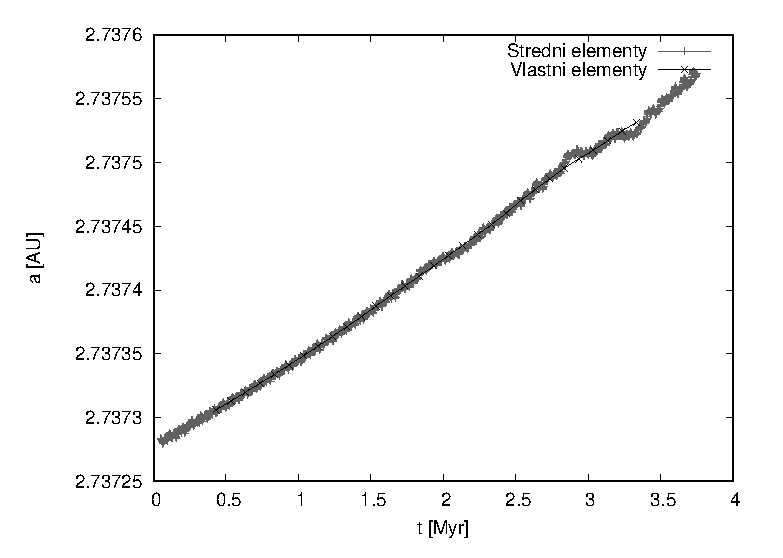
\includegraphics[width=0.8\textwidth]{obr/atFP}
	\caption{Porovnání střední hlavní poloosy $a_{\rm m}$ a vlastní $a_{\rm p}$ pro simulaci jedné planetky po dobu $3,76$ miliónů let. Lze vidět, že se za tuto dobu vlastní hlavní poloosa planetky zvýšila o~$\Delta a\doteq0.0002\,{\rm AU}\doteq30000\, {\rm km}$. Tento vývoj je způsoben Jarkovského jevem (viz~\ref{sec:jarko}), lze z grafu vyvodit, že tato planetka měla \I{prográdní} rotaci, neboť se její hlavní poloosa zvětšila.}
	\label{atFP}
\end{figure}

Vlastní elementy jsou elementy dráhy zbavené jak krátkých, tak dlouhých periodických perturbací, mezi které kromě již zmíněných patří navíc sekulární rezonance, které jsou způsobené závislostí frekvencí precese (změny) argumentu perihélia a délky vzestupného uzlu planetky a některé jiné planety nebo i vícero planet.

Vlastní elementy jsou tedy svým způsobem aritmetickými \uv{průměry} pohybu a jsou téměř neměnné na dlouhém časovém úseku, ačkoliv působením negravitačních sil --- především zmiňovaného Jarkovského jevu --- se můžou pomalu zvětšovat nebo zmenšovat. 

Mezi vlastní elementy počítáme pouze vlastní hlavní poloosu $a_{\rm p}$, vlastní excentricitu $e_{\rm p}$ a vlastní inklinaci $i_{\rm p}$. Ostatní elementy nemá cenu uvažovat, protože argument perihélia i délka vzestupného uzlu periodicky precedují (mění se v~intervalu $0^\circ$ až $360^\circ$) a střední anomálie je také přibližně lineárně závislá na čase (a to rychleji).

Výpočet vlastních se provádí pomocí Fourierovy analýzy, viz~\cite{sidlichovsky96}. 

\chapter{Planetky ve sluneční soustavě}


Podle Mezinárodní astronomické unie (IAU) se tělesa ve sluneční soustavě dělí především na planety, trpasličí planety, planetky, komety, přirozené satelity. Planeta je definována jako takové těleso, které obíhá kolem Slunce, není měsíc a má dostatečnou hmotnost, aby se ustavil přibližně kulovitý tvar, a \uv{vyčisťovalo} svoje okolí od ostatních těles. Kometa je pak těleso složené z~ledu a prachu, které většinou obíhá Slunce po excentrické dráze, vyhazuje \I{komu} (atmosféru) a zanechává za sebou \I{ohon}, což je způsobeno sublimací ledu z~komety a strháváním prachu působením slunečního záření. Další skupinou jsou trpasličí planety, kam v tuto chvíli patří pouze pět těles: Ceres, Pluto, Eris, Makemake, Haumea. Dále přirozené satelity jsou tělesa obíhající nějakou jiné těleso, různé od Slunce.

Zbývající skupinou jsou planetky, kam patří transneptunická tělesa (tj.\ obecný název tělesa, která se pohybují za oběžnou dráhou Neptunu), tělesa hlavního pásu planetek a jiná malá tělesa sluneční soustavy. Planetky můžeme dělit na podle jejich oběžné dráhy na tělesa vnitřní a vnější sluneční soustavy vzhledem k Jupiteru. Největší populace těles vnitřní soustavy se nachází v~hlavním pásu, který se nachází přibližně mezi $2,1\, {\rm AU}$ a $3,3\, {\rm AU}$ (viz obrázek~\ref{fig:belt}. Dále sem spadají také planetky, jejichž oběžná dráha protíná dráhu Marsu nebo Země --- blízkozemní planetky, a planetky nacházející se v~libračních bodech L4 a L5\footnote{To jsou takové body, v~nichž se vyrovnává působení gravitační a odstředivé síly. Jde tedy o~jakýsi bod rovnováhy. Body L4 a L5 se nacházejí na oběžné dráze většího tělesa o~$60^\circ$ \uv{napřed} nebo \uv{za} tělesem.} soustav Slunce--Země, Slunce--Mars, Slunce--Jupiter --- tj.\ příslušní Trojáné. Jako Hildy se označují planetky v rezonanci $3:2$ s Jupiterem. Dále se předpokládá existence Oortova oblaku, který se má nacházet za hranicí $1\,000\,{\rm AU}$ až do $100\,000\,{\rm AU}$ a který má být zdrojem dlouhoperiodických komet. Žádné těleso z této oblasti však ještě nebylo pozorováno.

\begin{figure}
	\centering
	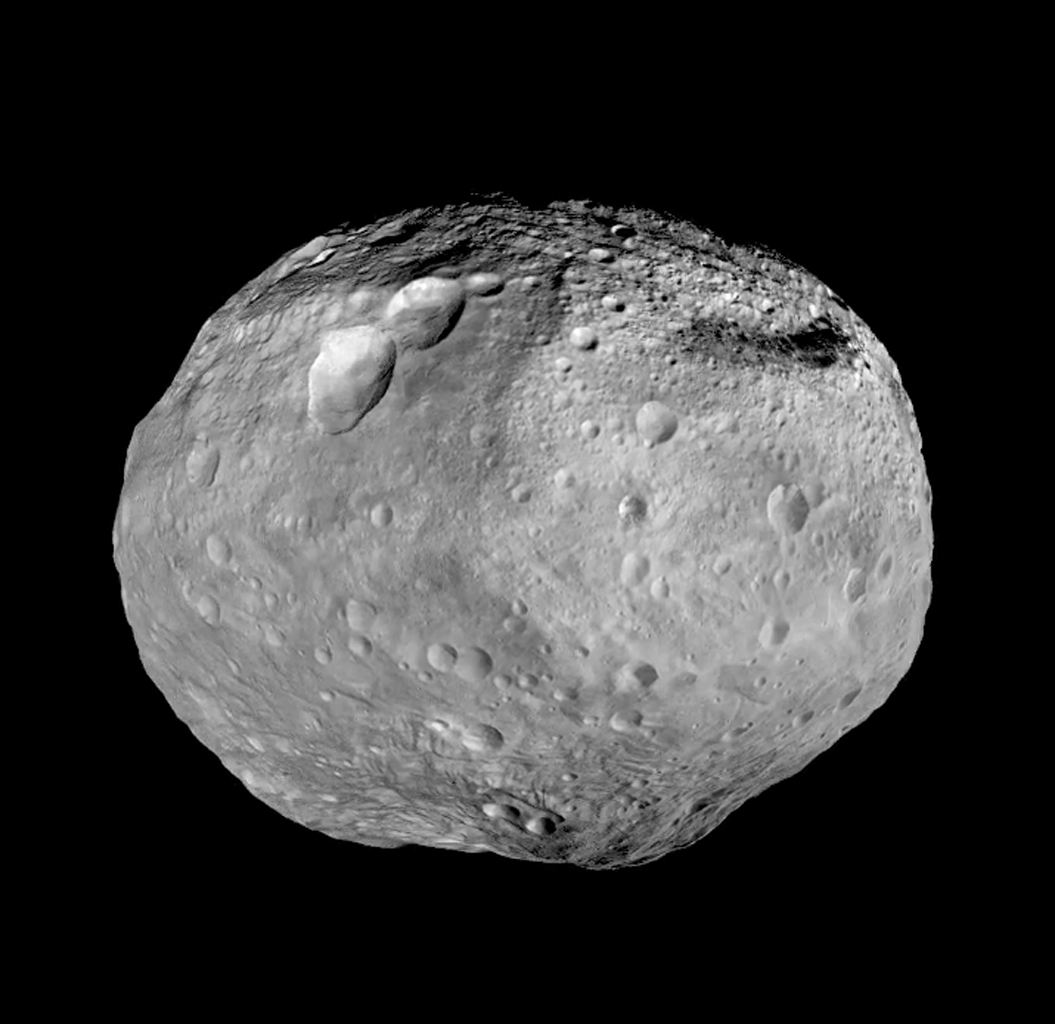
\includegraphics[width=0.6\textwidth]{obr/vesta.jpg}
	\caption{Planetka (4) Vesta, která je po trpasličí planetě (1) Ceres druhým největším a nejhmotnějším tělesem hlavního pásu planetek. Na jižní hemisféře lze pozorovat kráter Rheasylvia, který je jedním z největších ve sluneční soustavě. Fotografie byla pořízena sondou \I{Dawn}, jejíž cílem bylo i těleso (1) Ceres. Převzato z~\cite{jplvesta}.}
\end{figure}

Většina těles vnější sluneční soustavy se nachází v~Kuiperově pásu, který se sahá od oběžné dráhy Neptunu až do vzdálenosti přibližně $55\, {\rm AU}$. V nedávné době bylo americkou sondou \I{New Horizons} zblízka prozkoumáno jedno z těles této oblasti, \I{Ultima Thule}, které je v tuto chvíli nejvzdálenějším prozkoumaným objektem sluneční soustavy. Jedná se o dvojité kontaktní těleso (tj.\ má dvě pevně spojené kulovité části), které se zformovalo pravděpodobně při vzniku sluneční soustavy.~\cite{ultimathule}


\pagebreak
\section{Hlavní pás planetek}
Při našem studiu se budeme zaměřovat na planetky hlavního pásu, ve kterém se také nachází jediná trpasličí planeta ve vnitřní sluneční soustavě, Ceres, mající střední poloměr $473\, {\rm km}$. Ostatní pozorované planetky mají střední poloměr od $250\, {\rm km}$ po několik desítek metrů. Největší populace se rovnoměrně rozprostírá od vzdálenosti $2,1\, {\rm AU}$ od Slunce do vzdálenosti přibližně $3,3\, {\rm AU}$ a většina planetek má excentricitu menší než $0,4$ a sklon dráhy menší než $30^\circ$. Planetky, které vystoupí z~této oblasti (ať už zmenšením hlavní poloosy $a$ nebo zvětšením excentricity $e$), se buď přiblíží Marsu, Zemi nebo Venuši a jsou jejich gravitací vymrštěny na zcela odlišnou oběžnou dráhu, nebo se obdobně přiblíží Jupiteru, který též může výrazně změnit jejich původní oběžnou dráhu nebo může způsobit rozpad tělesa vlivem slapových jevů.

\begin{figure}
	\centering
	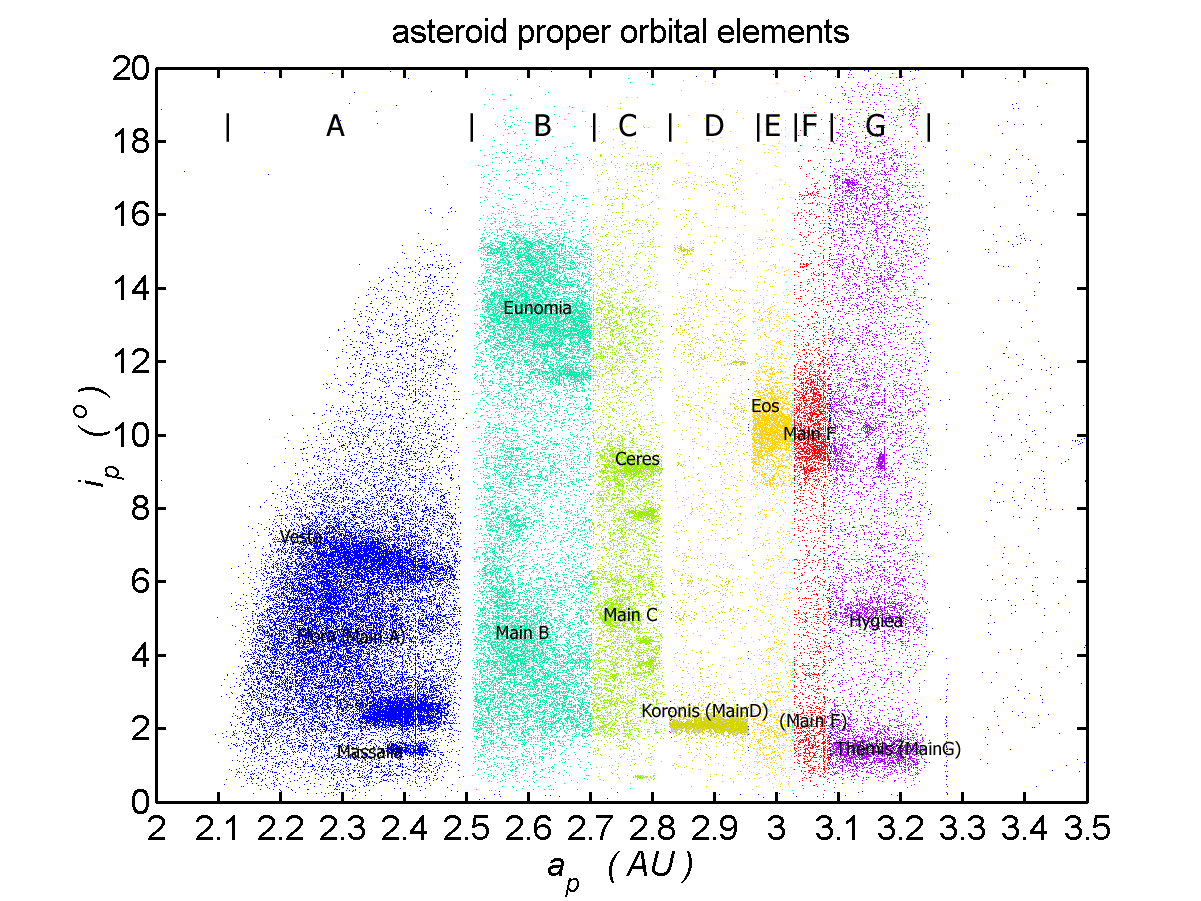
\includegraphics[width=0.9\textwidth]{obr/mainbelt.png}
	\caption{Planetky hlavního pásu podle vlastních elementů --- osa $x$ znázorňuje vlastní velkou poloosu a osa $y$ vlastní sklon. Lze vidět některé rodiny planetek, konkrétně uprostřed nahoře se nachází rodina Eunomia. Barevné označení znázorňuje oblasti mezi hlavními rezonancemi středního pohybu. Převzato z~\cite{wiki:belt}.} \label{fig:belt}
\end{figure}

\pagebreak
\section{Rezonance}
Struktura hlavního pásu planetek je významně ovlivněna rezonancemi, což jsou oblasti v~prostoru, ve kterém když se planetka nachází, je nějaký údaj o~její dráze a nějaké planety, běžně Jupitera nebo Saturnu, v~jednoduchém poměru, tedy ve zlomku s~nízkým čitatelem a jmenovatelem. Pro polohy sekulárních rezonancí jsou vztahy podstatně složitější, neboť závisejí na polohách a hmotnostech vícero planet.
\subsection{Rezonance středního pohybu} \label{sec:meanmotion}
%Nástin výpočtu jejich polohy (je to jednoduché), vysvětlení vlivu na HCM

Rezonance středního pohybu jsou nejjednodušším a obvykle také nejsilnějším typem rezonancí. Nastávají, když je oběžná doba planetky a planety v~poměru nízkých celých čísel, např. $3:2$ --- to znamená, že zatímco planetka dokončí tři celé oběhy, planeta vykoná dva a obě tělesa se znovu potkají na počáteční pozici. 

Vlivem těchto rezonancí se může hlavní poloosa planetky a excentricita periodicky měnit, podobně jako je tomu u kyvadla. Některé rezonance, resp.\ překryvy rezonancí postupně zvyšují excentricitu dráhy planetky, až se její perihélium dostane pod oběžnou dráhu nějaké vnitřní planety, např. Marsu nebo Země, což eventuálně způsobí vzájemné blízké přiblížení, které planetku vymrští na jinou oběžnou dráhu. Takto může planetka úplně opustit sluneční soustavu. Za určitých podmínek se perihélium planetky může snížit natolik, že překročí Rocheovu mez\footnote{což je hraniční vzdálenost od centrálního tělesa, kterou když planetka držená pohromadě pouze vlastní gravitací překročí, je vlivem slapové síly (rozdílu gravitačních sil) roztržena na malé kousky, které jsou soudržné díky elektromagnetickým silám.}, rozpadne se a úlomky jsou pohlceny hvězdou a stávají se její součástí~\cite{pichierri17}.

Výpočet umístění rezonance středního pohybu, tedy vzdálenosti od Slunce, je poměrně jednoduchý, uvádíme proto postup pro rezonanci ovlivňující rodinu Eunomia, kterou je rezonance $8:3$ s~Jupiterem. Vzpomeňme na Třetí Keplerův zákon, který říká
\begin{align} \label{eq:3kep}
	\frac{T_1^2}{T_2^2}=\frac{a_1^3}{a_2^3}\,, 
\end{align}
kde $T_1$, $T_2$ označují oběžné dvou tělesa a $a_1$, $a_2$ jejich hlavní poloosy. Předpokládejme, že v~námi hledané rezonanci $8:3$ se nachází nějaká planetka a vypočítejme délku její hlavní poloosy, a to úpravou rovnice~\eqref{eq:3kep} jako
\begin{align} \label{eq:3kepa}
	a_2=\left(\frac{T_2}{T_1}\right)^{\frac{2}{3}}a_1\,,
\end{align}
kde $T_1$, resp.\ $T_2$ zde značí oběžnou dobu Jupitera, resp.\ planetky, a $a_1$, resp.\ $a_2$ délku hlavní poloosy Jupitera, resp.\ planetky. Oběžná doba Jupitera je přibližně $4332,59\,$dnů a délka jeho hlavní poloosy přibližně $5,203\,{\rm AU}$. Protože hledáme rezonanci $8:3$, musí platit $\frac{T_2}{T_1}=\frac{3}{8}$. Po dosazení do rovnice~\eqref{eq:3kepa} dostáváme $a_2=2,706\,{\rm AU}$, což lze dobře ověřit na obrázku~\ref{fig:ae_ai_wise} rozdělení rodiny Eunomia v~prostoru hlavní poloosy a excentricity.
\subsection{Sekulární rezonance} 
Sekulární rezonance jsou sice obvykle mírnějšího rázu než rezonance středního pohybu, ale na dlouhodobý vývoj hlavního pásu mají značný vliv. Slovo sekulární pochází z~latinského \I{saeculum}, což znamená století nebo generace, což odkazuje na dlouhodobý charakter sekulárních rezonancí. Veličiny, které zde dáváme do poměru, jsou rychlosti precese argumentu perihélia $\omega^\prime$ a rychlosti precese délky vzestupného uzlu $\Omega^\prime$, které ovšem závisejí na velké poloose planetky a jejích vzdálenostech od všech planet. Proto pro jejich polohu neexistuje jednoduchý předpis (viz kap. 7 v~\cite{murray00}).

\pagebreak
\section{Rodiny planetek}

Rodiny planetek jsou skupiny těles, mající podobné charakteristiky, předně podobné vlastní elementy dráhy. Při jejich identifikaci musíme ale přihlížet i k ostatním veličinám, jako jsou albedo, barevné indexy, nebo reflexní spektrum. 

\immediate\write18{convert -trim obr/trajec_001.png obr/trajec_001t.png}
\immediate\write18{convert -trim obr/trajec_101.png obr/trajec_101t.png}
\immediate\write18{convert -trim obr/trajec_201.png obr/trajec_201t.png}
\immediate\write18{convert -trim obr/trajec_501.png obr/trajec_501t.png}
\begin{figure}
	\centering
	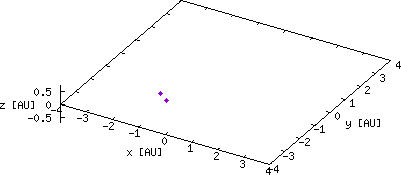
\includegraphics[width=0.49\textwidth]{obr/trajec_001t.png}
	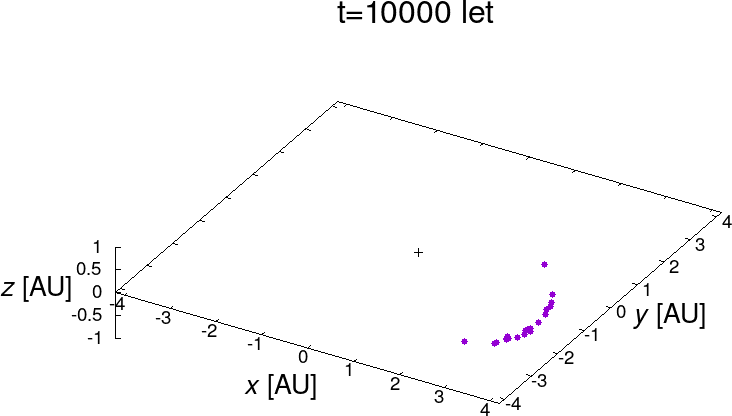
\includegraphics[width=0.49\textwidth]{obr/trajec_101t.png} \\
	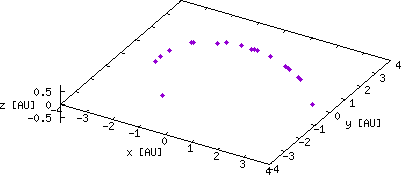
\includegraphics[width=0.49\textwidth]{obr/trajec_201t.png}
	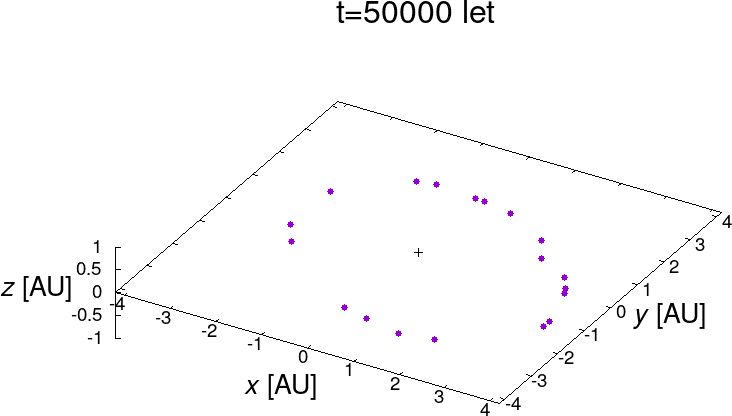
\includegraphics[width=0.49\textwidth]{obr/trajec_501t.png}
	\caption{Trojrozměrné polohy $x,\,y,\,z$ několika těles ($N=20$) ze simulované rodiny Eunomia rušené čtyřmi planetami (Jupiterem, Saturnem, Uranem a Neptunem) v~časech $t=0,\,10\,000,\,20\,000,\,50\,000\,{\rm let}$ po úvodním izotropním rozpadu. V čase $t=0$ měla všechna tělesa stejnou polohu $x,\,y,\,z$, ale různé rychlosti $v_x,\,v_y,\,v_z$, tedy i různé elementy dráhy, především hlavní poloosu, díky čemuž se lišily i jejich oběžné doby, které se pohybují kolem $4,27$ let. Po $50\,000$ letech lze pozorovat rozprostření podél dráhy ve střední anomálii $M$, což je element, který je nejsnáze měněn perturbacemi.} \label{fig:trajec}
\end{figure}

Rodiny vznikají srážkou dvou planetek, čemuž v~závislosti na poměru velikosti mateřského tělesa a projektilu říkáme buď \I{katastrofický rozpad} (\uv{na malé úlomky}), \I{reakumulační rozpad} (úlomky se působením gravitace \uv{slepí} zpátky) nebo \I{kráterování}. Může se zdát, že srážky jsou v~tak rozlehlém prostoru jako je sluneční soustava velmi málo pravděpodobné, ale v~dlouhém časovém úseku --- $4,5\,\text{miliardy let}$ od vzniku naší sluneční soustavy --- k~srážkám dochází, a mají nejenom vliv na vznik rodin, ale také na jejich následný vývoj (vzniklé fragmenty se spolu nadále srážejí).

Rodiny planetek, které již prošly dlouhodobým vývojem, se samozřejmě na obloze nejeví jako skupina společně letících planetek, kvůli rozdílné velké poloose $a$, resp.\ oběžné době $T$ se totiž záhy rozptýlí ve střední anomálii $M$, jak lze vidět na obrázku~\ref{fig:trajec}.

\subsection{Metody identifikace rodin} \label{sec:metodyiden}
Nejpoužívanější metodou pro identifikaci rodin planetek je \I{hierarchická shlukovací metoda} (HCM) \cite{zappala90}. Spočívá v~tom, že si v~trojrozměrném prostoru vlastních elementů ($a_{\rm p},\,e_{\rm p},\,i_{\rm p}$) zvolíme metriku --- veličinu, kterou budeme popisovat vzdálenost dvou těles, a poté, pomocí zvolené hraniční \I{vzájemné} vzdálenosti, určíme, která tělesa patří do rodiny. Tato metrika má přitom jednotku rychlosti, aby ji bylo možné porovnávat s rychlostmi výhozu fragmentů. Je určena vztahem
\begin{align}
	v=na_{\rm p}\sqrt{C_a\left(\frac{\Delta a_{\rm p}}{a_{\rm p}}\right)^2+C_e(\Delta e_{\rm p})^2+C_i(\Delta \sin i_{\rm p})^2}\,,
\end{align}
kde $n$ značí střední pohyb, dále pokud označíme $1$ a $2$ tělesa, mezi kterými vzdálenost počítáme, platí $a_{\rm p}=(a_{{\rm p}1}+a_{{\rm p}2})/2$ (kvůli symetrii) a $\Delta a_{\rm p}=a_{{\rm p}1}-a_{{\rm p}2}$, $\Delta e_{\rm p}=e_{{\rm p}1}-e_{{\rm p}2}$ a $\Delta \sin i_{\rm p}=\sin i_{{\rm p}1}-\sin i_{{\rm p}2}$; $C_a,\,C_e,\,C_i$ jsou váhy, které přiřazujeme jednotlivým elementům, přičemž možnou a i v~této práci použitou volbou je $C_a=5/4$, $C_e=2$, $C_i=2$~\cite{zappala90}. 

Samotný průběh tohoto algoritmu je jednoduchý: zvolíme nějakou hraniční rychlost $v_{\rm cutoff}$ a poté, většinou počínaje největším tělesem, např. (15) Eunomia, hledáme dvojice těles, pro které je $v<v_{\rm cutoff}$; vždy když nějakou nalezneme, přidáme si ji do seznamu zkoumané rodiny a postup opakujeme, dokud nám nepřibývají žádní noví členové. Výsledný počet členů je samozřejmě závislý na volbě $v_{\rm cutoff}$, což lze vidět na obrázku~\ref{fig:Nv}.

Jak ukážeme později v~této práci (kap.~\ref{sec:interlopers}), tato metoda samotná nestačí ke kompletní identifikaci rodiny, neboť musíme odstranit \I{přimísená tělesa} (angl.\ interlopers), např.\ porovnáním albed (viz obrázek~\ref{fig:pV_pIR}), barevných indexů (viz obrázek~\ref{fig:astar_iz}), grafu závislosti hlavní poloosy a hvězdné velikosti, případně dalšími metodami závisejícími na konkrétní situaci v okolí rodiny.

\subsection{Nevratné děje při vývoji}
%Disipační síly, vliv na vývoj v~prostoru vlastních elementů, reference na nějaký článek o~nové databázi tvarů planetek???

Doteď jsme se zabývali pouze silami, které vznikají vzájemným gravitačním působením těles, nejenom ve sluneční soustavě ale působí i několik dalších sil, týkajících se zejména emise tepla. Společně s náhodnými srážkami a chaotickou difuzí tvoří tyto jevy nevratné děje při vývoji planetek a komet, se kterými je při jejich studiu nutno počítat.

\subsubsection{Jarkovského jev} \label{sec:jarko}
Jarkovského jev, který je pojmenován po Ivanu Ospichovi Jarkovskému\footnote{Jarkovský ale tento jev nepopsal úplně stejně, jako ho chápeme teď; v tehdejší době byla ještě populární teorie o éteru --- všudypřítomném médiu --- a právě této látce Jarkovský připisoval ono zpomalování nebo zrychlování těles. Tím \enquote{správným} způsobem popsali tento jev nezávisle Ernst Julius Öpik (1893--1985) a Vladimir Vyacheslavovich Radzievskii (1911--2003)~\cite{brozphd}.}  (1844--1902), je nejdůležitější negravitační silou, která ovlivňuje strukturu hlavního pásu planetek. Jejím působením se totiž tělesa posouvají v hlavní poloose, čímž se dostávají do oblastí rezonancí, které pak mohou jejich pohyb nadále ovlivnit.

\begin{figure} 
	\centering

		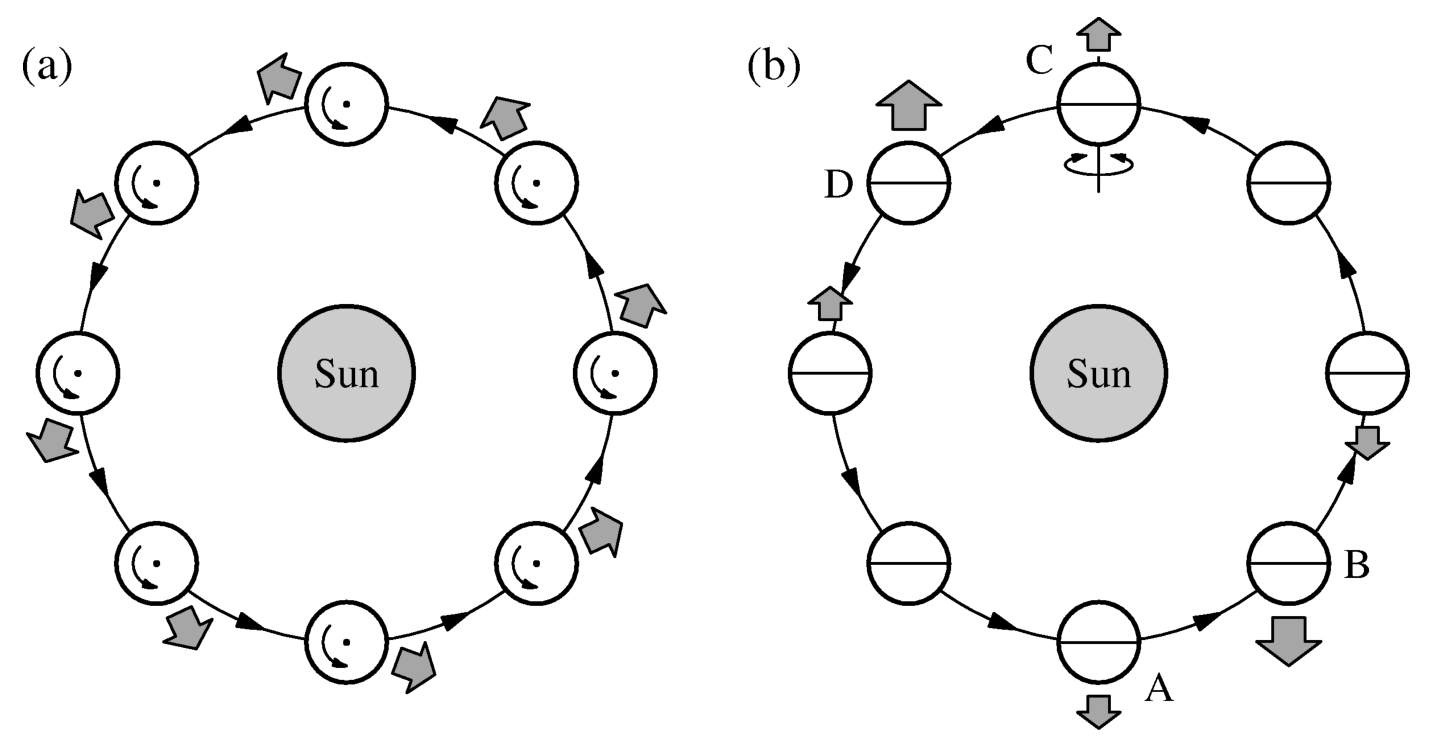
\includegraphics[width=0.8\textwidth]{obr/jarkovskeho_jev.png}
	\caption{Denní a roční varianta Jarkovského jevu. Šedivé šipky
	označují zbytkovou sílu, která působí na těleso. (a) Denní Jarkovského jev, když se těleso otáčí kolem osy kolmé k oběžné dráze. V tomto případě se těleso natočí teplejší stranou vždy \uv{za sebe}, tepelná emisí pak vzniká zbytková síla, jejíž jedna složka působí ve směru pohybu tělesa, velká poloosa se tedy bude zvětšovat. (b) Roční Jarkovského jev, s rotační osou ležící v orbitální rovině. Ohřívání přivrácené polokoule, zejména v bodech A a C, a opožděná emise tepelného záření, zvláště v bodě B a D, způsobují zbytkovou sílu, jejíž jedna složka směřuje proti pohybu tělesa, tudíž velká poloosa se bude zmenšovat. Převzato z~\cite{fmt}.} \label{fig:jarko}
\end{figure}

Rozlišujeme dvě varianty Jarkovského jevu --- denní a roční. Jejich rozdíl je popsán v~\ref{fig:jarko}. Výsledná změna hlavní poloosa je samozřejmě důsledkem kombinace obou variant, pro tělesa s hodnotou šikmosti (obliquity)\footnote{Obliquita je úhel mezi rotační osou tělesa a kolmicí k dráze, obliquita $0^\circ$ a $180^\circ$ značí rotační osu kolmou na ekliptiku, přičemž $0^\circ$ je tzv.\ prográdní rotace (těleso vlivem Jarkovského efektu zrychluje) a $180^\circ$ tzv.\ retrográdní rotace (těleso zpomaluje)} blízko $0^\circ$ nebo $180^\circ$ dominuje denní varianta, zatímco pro obliquitu kolem $90^\circ$ je roční varianta silnější. Dále pro tělesa s rychlejší rotační periodou (řádově menší než oběžná doba) je silnější denní varianta, a pro tělesa s delší rotační periodou roční varianta. 

Jarkovského jev byl poprvé pomocí radarů změřen v roce 2003 při zkoumání pohybu blízkozemní planetky (6489) Golevka.~\cite{chesley03}
\subsubsection{YORP jev}
%Popis,  zesílení Jarkovského jevu

Yarkovsky–O'Keefe–Radzievskii–Paddack jev je stejně jako Jarkovského jev důsledkem nerovnoměrného rozložení a emise tepla tělesa, YORP však funguje pouze pro nesférická tělesa. Jeho účinkem je zvětšování úhlové rychlosti rotace $\omega$ a zmenšování obliquity $\theta$ a je způsoben nepravidelným povrchem planetky, který vyzařuje teplo nerovnoměrně. V dlouhém časovém měřítku YORP \enquote{táhne} úhlovou rychlost buď k $0$, nebo k nekonečnu a obliquitu buď ke $0^\circ$ nebo ke $180^\circ$. Protože Jarkovského jev je nejsilnější právě pro tyto hodnoty obliquity, funguje YORP jako takový \uv{zesilovač} Jarkovského jevu. 

Jak YORP, tak Jarkovského jev je silnější pro menší tělesa. Na ty úplně nejmenší tělesa, prachové částice, působí \I{Poynting-Robertsonův efekt}\footnote{Vzájemný pohyb částice a Slunce způsobuje, že sluneční záření dopadá na částici pod úhlem jiným než $90^\circ$ vzhledem k pohybu částice, čímž částici zpomaluje.}, který způsobuje postupné zpomalování částice až dojde ke kolizi se Sluncem samotným. 

\subsubsection{Náhodné srážky}
Po úvodní srážce se tělesa zpět reakumulují do větších kusů, které nadále letí po heliocentrických drahách, a je zřejmé, že v dlouhém časovém úseku se některá z nich srazí s nějakým jiným tělesem. Tím vznikají další menší tělesa, jejichž rotační osa a doba je navíc různá od původního tělesa, což má vliv na Jarkovského a YORP jev. 

\subsubsection{Chaotická difuze}
Je známo, že dvojité (i vícenásobné) kyvadlo se chová chaoticky, tedy jeho stav je velmi náchylný k drobným změnám počátečních podmínek. To ale neznamená, že jeho vývoj nemůžeme simulovat, jedná se totiž o \I{deterministický chaos}. Jak jsme zmiňovali v~\ref{sec:meanmotion}, dráhové rezonance se chovají podobně jako kyvadlo, a proto, když se rodina nachází blízko překryvu dvou nebo více rezonancí, můžou někteří její členové tuto oblast chaoticky opustit. Tento děj je v podstatě nevratný, protože takový chaotický systém nelze rozumně zpětně integrovat.

\chapter{Vlastnosti rodiny Eunomia} \label{ch:eunomia}
% Postup určování rodiny, volba $v_{cutoff}$, pozadí --- [česky???] interlopers (ref na později), rozdělení velikostí 
Rodina Eunomia se nachází se v centrálním pásu planetek --- mezi $2,5\,{\rm AU}$ a $2,82\,{\rm AU}$ a patří mezi nejstarší rodiny vůbec. Její členové včetně největšího tělesa jsou taxonomického typu S, což znamená, že se převážně skládají z křemičitanů. Existují ale i návrhy, že původní mateřské těleso nebylo homogenní~\cite{nathues05}, ale částečně diferenciované, což by mohlo způsobit zvýšení počtu členů této rodiny.

Rozšířit! Informace o prvním objevení.???

\section{Identifikace členů}

V této práci byla k identifikaci členů rodiny Eunomia použita \textit{hierarchická shlukovací metoda}, popsaná v části~\ref{sec:metodyiden}. Závislost počtu členů rodiny na hraniční rychlosti lze vidět na obrázku~\ref{fig:Nv}. Můžeme pozorovat, že rodina Eunomia je dobře oddělená od ostatních rodin --- jedinou blízkou rodinou je rodina Adeona, jejíž planetky ale nejsou součástí rodiny Eunomia. K dalším výpočtům jsme použili hodnotu $v_{\rm cutoff}=44\,{\rm m/s}$, při které počet členů rodiny před odstraněním přimísených těles činil 6503.

\begin{figure}
	\centering
	\includegraphics[width=0.6\textwidth]{obr/Nv}
	\caption{Závislost počtu členů rodiny Eunomia na zvolené hraniční rychlosti $v_{\rm cutoff}$ při výpočtu HCM\@. Počet členů prudce vzroste při přechodu z~rychlosti $43\,{\rm m/s}$ na $44\,{\rm m/s}$, což je způsobené poměrně velkou vzdáleností prvního nejbližšího tělesa od mateřského (15) Eunomia. Dále vzroste prudce při přechodu z~rychlosti $46\,{\rm m/s}$ na $47\,{\rm m/s}$, což je způsobené splynutím s~rodinou Adeona.}
	\label{fig:Nv}
\end{figure}

\subsection{Přimísená tělesa} \label{sec:interlopers}
%Odstranění interlopers, barevné indexy, SLOAN, WISE, ref na Nejistoty veřejných dat.

Prvním mechanismem k odstranění přimísených těles je graf závislosti vlastní velké poloosy $a_{\rm p}$ a \textit{absolutní hvězdné velikosti} $H$ \footnote{\textit{Absolutní hvězdná velikost} neboli \textit{magnituda} $H$ je taková \textit{zjevná hvězdná velikost}, kterou by těleso mělo, kdyby bylo vzdálené 10 parseků (jeden parsek je vzdálenost, z níž má 1 astronomická jednotka úhlovou velikost 1 vteřiny), neboli přibližně 32,6 světelných let. Obecně pro hvězdné velikosti platí Pogsonova rovnice
\begin{align*}
	M_2-M_1=-2,5\log\left(\frac{L_2}{L_1}\right)\,,
\end{align*}
kde $L_1$ a $L_2$ označují zářivé výkony těles. Podle definice se bere, že hvězda s $L_0=3,055\cdot10^{28}\,{\rm W}$ má $M=0$, tedy absolutní hvězdná velikost $H$ se spočte jako
\begin{align*}
	H=0-2,5\log\left(\frac{L}{L_0}\right)\,,
\end{align*}
přičemž zjevnou hvězdnou velikost $m$ můžeme vypočítat jako
\begin{align*}
	m=5(\log d -1)-2,5\log\left(\frac{L}{L_0}\right)\,,
\end{align*}
kde $d$ označuje vzdálenost tělesa od pozorovatele v parsecích.~\cite{fmt}} 
(obrázek~\ref{fig:aH_wise}), na kterém lze pozorovat vliv Jarkovského jevu a YORPu. Platí, že unášení v hlavní poloose je větší pro menší tělesa, protože obsah povrchu planetky, kterému je úměrná síla Jarkovského jevu, roste s druhou mocninou poloměru, zatímco objem, kterému je úměrná hmotnost, roste s třetí mocninou poloměru. Tím lze odstranit tělesa, která se vzhledem k jejich hvězdné velikosti nemohla po původním rozpadu dostat na grafu $(a_{\rm p},\,H)$ tam, kde jsou. Tuto závislost lze modelovat funkcí 
\begin{align}
	H=5\log\left(\frac{\Delta a_{\rm p}}{C}\right)\,,
\end{align}
kde $H$ označuje absolutní magnitudu, $\Delta a_{\rm p}$ vzdálenost v hlavní poloose od středu rodiny a $C$ parametr, který záleží na naší volbě. Běžně se jako střed rodiny bere největší těleso, v našem případě jsme ale byli nuceni celou funkci o něco posunout, aby lépe seděla na ostatní pozorované objekty. Zvolené hodnoty můžete najít v popisku obrázku~\ref{fig:aH_wise}.
\begin{figure}
	\centering
	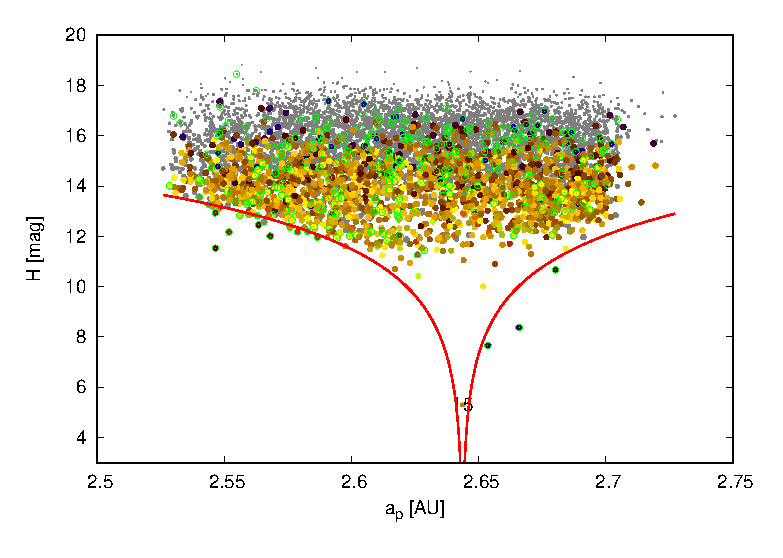
\includegraphics[width=0.7\textwidth]{obr/aH_wise}
	\caption{Rozdělení pozorované rodiny Eunomia v~rovině vlastní hlavní poloosy $a_{\rm p}$ a absolutní hvězdné velikosti $H$. Barevná škála byla převzata z katalogu WISE. Šedá křivka označuje funkci s parametry ${C=2,2\cdot10^{-4}}$ a ${a_c=2,643666\,{\rm AU}}$ a červená křivka označuje posunutou funkci s parametry ${C=2\cdot10^{-4}}$ a ${a_c=2,641666\,{\rm AU}}$. K odstranění  jsme zvolili červenou funkci. Lze pozorovat typický tvar \uv{V}, který je způsobem počátečním rychlostním polem a Jarkovského jevem, jenž je navíc ještě zesílen vlivem YORPu, což způsobuje zvýšenou koncentraci malých planetek na okrajích rodiny.}
	\label{fig:aH_wise}
\end{figure}

Další metodou k odstranění přimísených těles jsou metody spektroskopické, tedy zkoumající světelné charakteristiky těles. První z nich je graf závislosti albed\footnote{Geometrické albedo je poměr zářivosti tělesa ku zářivosti ideálního bezztrátového disku o stejném průřezu.~\cite{fmt}} $p_{\rm V}$, resp. $p_{\rm IR}$ ve viditelném, resp.infračerveném spektru. Pokud uvažujeme, že původní těleso bylo homogenní, měly by všechny vzniklé úlomky mít podobné albeda, čímž lze vyřadit tělesa, která očividně nemohla vzniknout ze stejného mateřského tělesa. Závislost $(p_{\rm V},\,p_{\rm IR}$) lze vidět na obrázku~\ref{fig:pV_pIR}, v jehož popisku lze také najít zvolené krajní hodnoty, které jsme zvolili pouze pro albedo $p_{\rm V}$, protože albedo $p_{\rm IR}$ je mu přímo úměrné.

\begin{figure}
	\centering
	\includegraphics[width=1.0\textwidth]{obr/pV_pIR}
	\caption{Albeda $p_{\rm V}$ (ve viditelném spektru) a $p_{\rm IR}$ (v infračerveném spektru) z~katalogu WISE \cite{nugent15}. Barevná škála byla taktéž převzata z katalogu WISE, barvy neodpovídají reálnému zbarvení. Zelené kroužky označují přimísená tělesa vyřazená jakoukoliv z použitých metod. Pro vyřazení přimísených těles touto metodou byly zvoleny hraniční hodnoty $0,05 \leq p_{\rm V} \leq 0,4$.}
	\label{fig:pV_pIR}
\end{figure}

Podobně jako předtím můžeme identifikovat přimísená tělesa pomocí jejich barevných indexu $a^*$ a $i-z$ tentokrát z katalogu SLOAN, který používá fotometrický systém skládající se z pěti filtrů $u,\,g,\,r,\,i,\,z$, přičemž každý z nich propouští světlo o dané vlnové délce. Zmíněné veličiny 
$u,\,g,\,r,\,i,\,z$ pak označují intenzitu světla o této vlnové délce. Veličina $a^*$ je definována vztahem~\cite{ivezic01}
\begin{align}
	a^ *= 0,89 (g - r) + 0,45 (r - i) - 0,57\,.
\end{align}
\begin{figure}
	\centering
	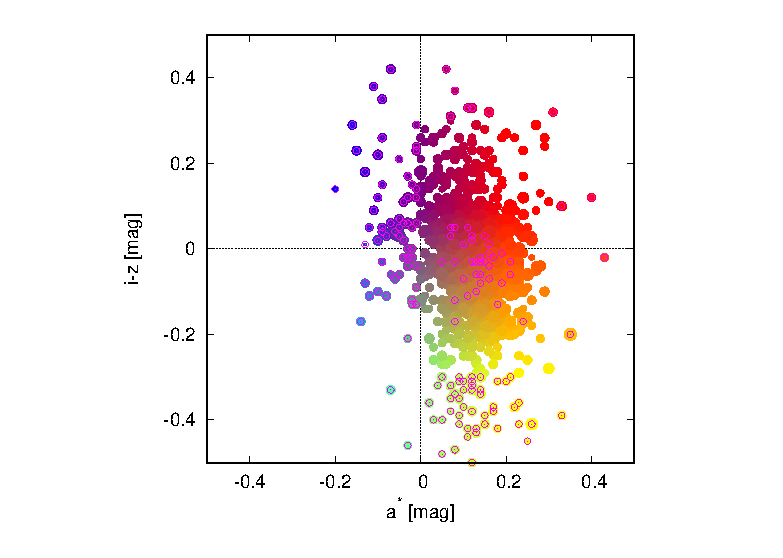
\includegraphics[width=1.0\textwidth]{obr/astar_iz}
	\caption{Barevné indexy $a^*$ a $i-z$ z~katalogu SLOAN \cite{ivezic01}. Barevná škála byla taktéž převzata z katalogu WISE, barvy neodpovídají reálnému zbarvení. Zelené kroužky označují přimísená tělesa vyřazená jakoukoliv z použitých metod. Pro vyřazení přimíšených těles byly zvoleny hraniční hodnoty $0\leq a^* \leq 0,3$ a $-0,3\leq i-z \leq 0,3$.}
	\label{fig:astar_iz}
\end{figure}
\pagebreak

\section{Fyzikální model pro rodinu Eunomia}
%Rozdělení v~$ae$ a $ai$ prostoru, vliv rezonancí J8/3 a J13/5, Gaussovy rovnice --- elipsa, volba bodu rozpadu ($f=90^o$, $\omega+f=50^o$).

Část o SFD napsat až po vytvoření syntetických SFD (pro porovnání)???
\begin{figure}
	\centering
	\begin{subfigure}[b]{0.45\textwidth}
	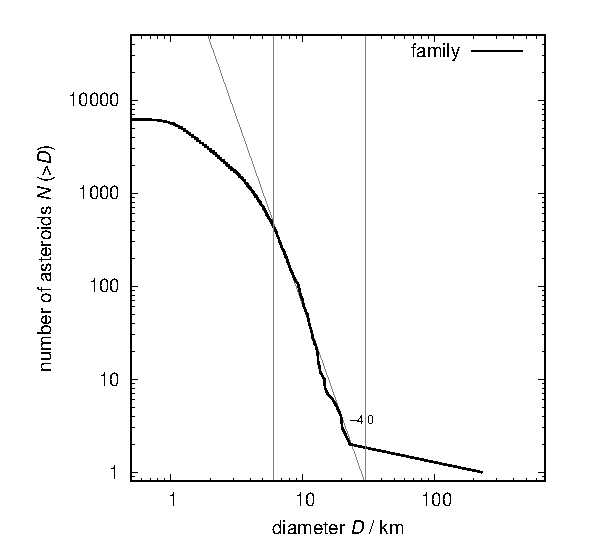
\includegraphics[width=\textwidth]{obr/size_distribution}
	\end{subfigure}
	\begin{subfigure}[b]{0.45\textwidth}
	\includegraphics[width=\textwidth]{obr/size_distribution_SMALLD}
	\end{subfigure}
	\caption{Histogram četnosti velikostí planetek rodiny Eunomia pro $v_{\rm cutoff}=44\,{\rm m/s}$, kde veličina $N({>}D)$ označuje počet planetek s~průměrem větším než $D$. Jedná se o logaritmický graf $(\log D,\,\log N({>}D))$.}
	\label{size_distribution}
\end{figure}
\subsection{Rozdělení v prostoru $(a,\,e)$ a $(a,\,i)$}
Jedním z nejdůležitějších úkonů, které je nutno provést před spuštěním simulace orbitálního vývoje, je správně určit, kde nastal úvodní rozpad (určit hodnoty $f$ a $\omega+f$), to totiž může významně ovlivnit rozdělení rodiny na grafech vlastní hlavní poloosy $a_{\rm p}$ versus vlastní excentricita $e_{\rm p}$ (prostor $(a,\,e)$) nebo versus vlastní sklon $\sin I_{\rm p}$ (prostor $(a,\,i)$). Na obrázku~\ref{fig:ae_ai_wise} můžeme vidět pozorovanou rodinu Eunomia společně s elipsami, které korespondují s rozdělením rodiny při rozpadu na různých místech. Tyto elipsy jsou určeny Gaussovými rovnicemi: pokud na těleso na působí zrychlení $\vec{a}=(R,\,T,\,W)$, kde $R$ označuje radiální složku (podél spojnice s centrálním tělesem), $T$ transverzální složku (podél tečny k oběžné dráze po směru oběhu) a $W$ normálovou složku (kolmou na rovinu oběhu), budou se elementy dráhy tělesa měnit jako
\begin{align}
	\diff{a}{t}&=\frac{2}{n\sqrt{1-e^2}}\left[T+e(T\cos f+R\sin f)\right] \,, \\
	\diff{e}{t}&=\frac{\sqrt{1-e^2}}{na}\left[R\sin f+T(\cos f+\cos E)\right]\,, \\
	\diff{I}{t}&=\frac{W}{na\sqrt{1-e^2}}\frac{r}{a}\cos(\omega+f)\,,
\end{align}
kde $a$ označuje hlavní poloosu, $e$ excentricitu, $I$ sklon, $n$ střední pohyb, $f$ pravou anomálii, $E$ excentrickou anomálii (viz obrázek~\ref{fig:E}), $\omega$ argument pericentra (viz obrázek~\ref{fig:elip}) a $r$ vzdálenost od centrálního tělesa. Převzato z~\cite{fmt}.

Jak můžeme vidět jak v Gaussových rovnic, tak na obrázku~\ref{fig:ae_ai_wise}, na hlavní poloosu a excentricitu má vliv pouze hodnota $f$, zatímco na sklon má vliv pouze hodnota $\omega+f$. Pomocí vizuální kontroly s pozorovanou rodinou v prostorech $(a,\,e)$ a $(a,\,i)$ byly zvoleny hodnoty $f=90^\circ$ a $\omega+f=50^\circ$.
\begin{figure}
	\centering
	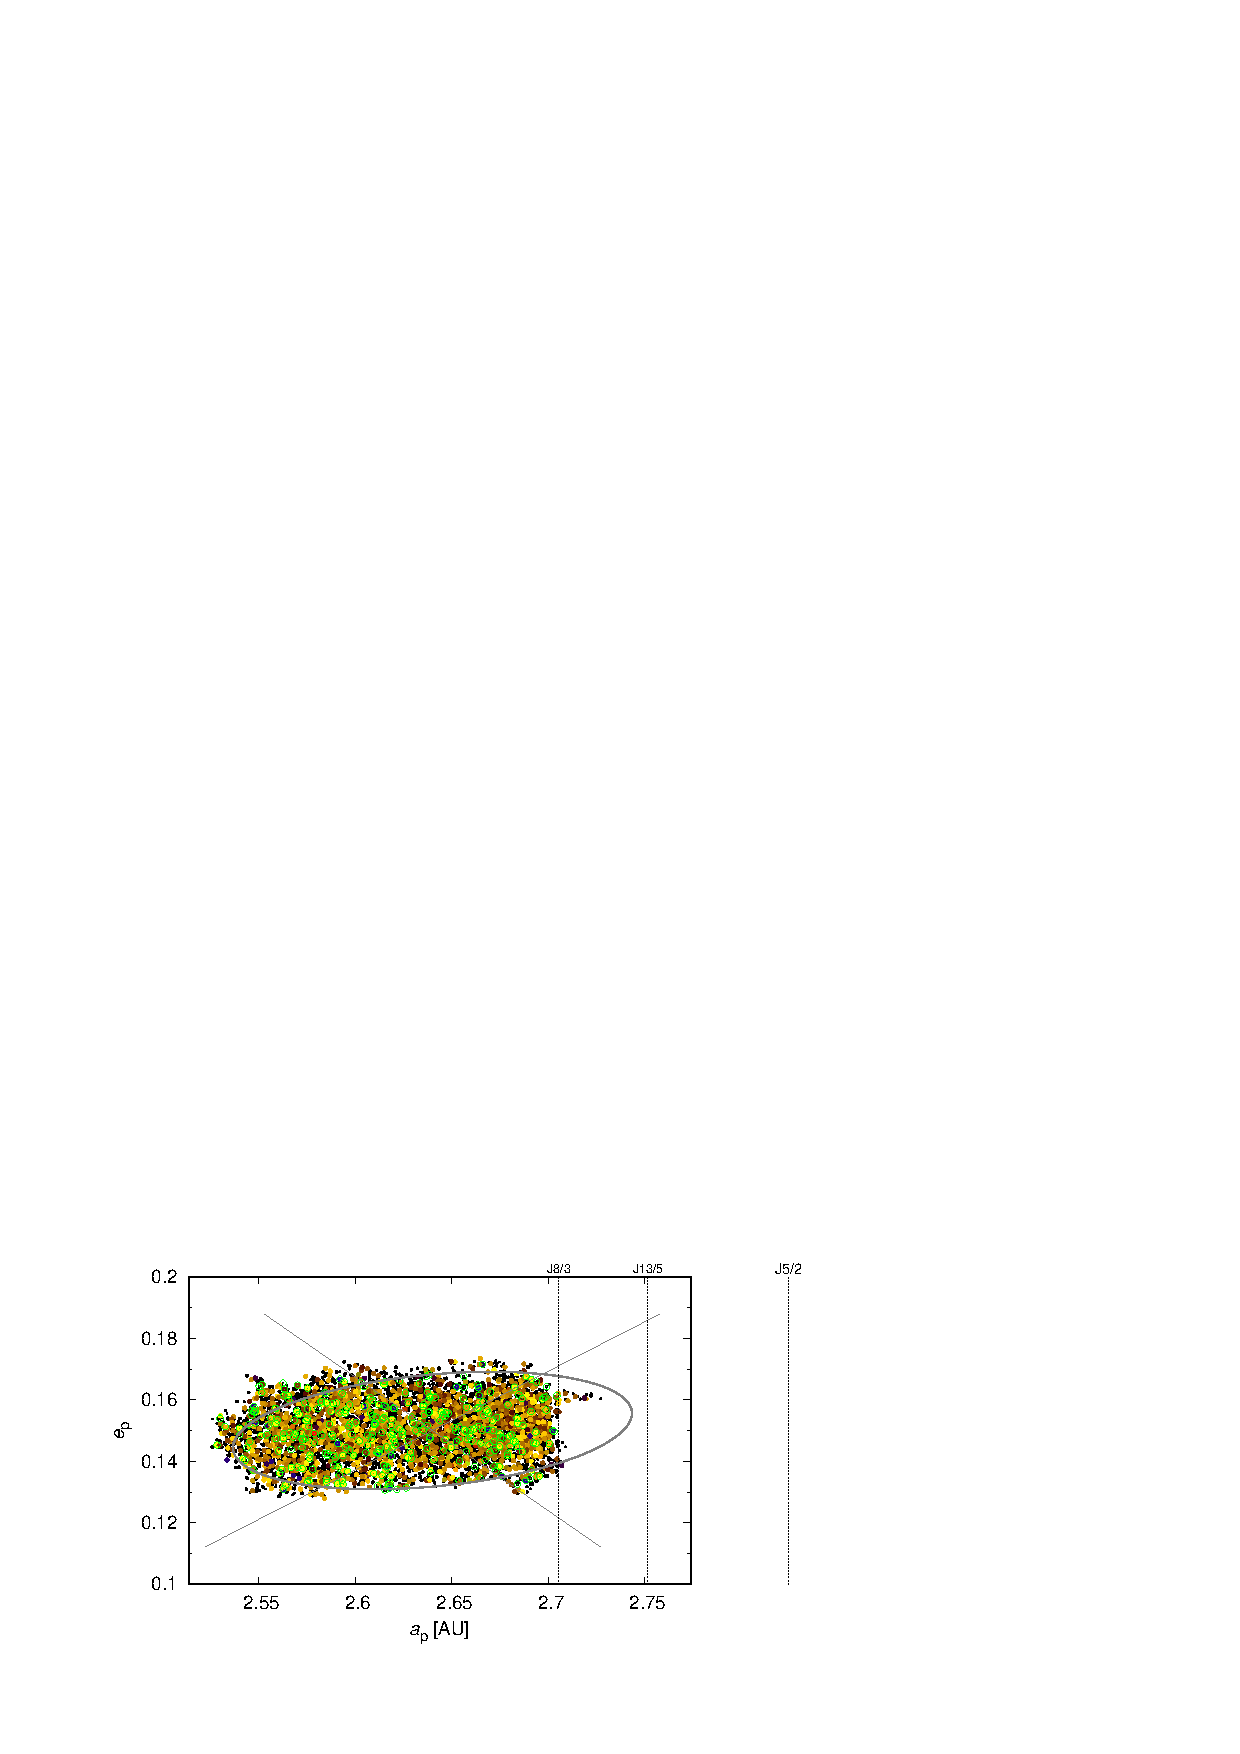
\includegraphics[width=0.8\textwidth]{obr/ae_wise}
	\includegraphics[width=0.8\textwidth]{obr/ai_wise}
	\caption{Pozorovaná rodina Eunomia v~rovině vlastní hlavní poloosy $a_{\rm p}$ a vlastní excentricity $e_{\rm p}$ (nahoře) a v~rovině vlastní hlavní poloosy $a_{\rm p}$ a vlastního sklonu $\sin I_{\rm p}$ (dole). Barevná škála odpovídá albedu $p_{\rm V}$ a $p_{\rm IR}$ z~katalogu WISE\@. Nápisy J8/3 a J13/5 označují polohu rezonancí středního pohybu s~Jupiterem. Šedé elipsy a úsečky (zdegenerované elipsy) naznačují výpočet Gaussových rovnic pro hodnoty pravé anomálie $f=0^\circ,\,90^\circ,\,180^\circ$ (nahoře) a $\omega+f=0^\circ,\, 50^\circ,\, 90^\circ$ (dole), kde zvolenou tučnější elipsou je elipsa pro hodnoty $f=90^\circ$ a $\omega+f=50^\circ$.}
	\label{fig:ae_ai_wise}
\end{figure}
\section{Nejistoty pozorovaných dat}
Nevím, nepsat???

\pagebreak
\section{Simulace orbitálního vývoje}
Konečně se dostáváme k části, kde budeme vlastní rodinu Eunomia simulovat po mnoho miliónů let. Krátkodobý výpočet problému $N$ těles byl proveden k vytvoření obrázku~\ref{fig:trajec}, nicméně takový výpočet nám neříká nic zajímavého o dynamické struktuře rodiny Eunomia a o jejím stáří. K těmto účelům se musí rodina simulovat po několik (přesněji 4) miliard let a posléze analyzovat její vzhled v prostorech $(a,\,e)$ a $(a,\,i)$ a její rozdělení velikostí.

\subsection{Dlouhodobé simulace}
%Popis experimentu (údaje o~výpočetní technice)
K dlouhodobé simulaci používáme upravený balíček SWIFT \cite{levison94}, s přidanými výpočty pro denní i roční Jarkovského jev, YORP efekt, náhodné srážky (kolizní reorientace os), úbytek hmoty způsobený otáčením tělesa a filtry k výpočtu středních a vlastních elementů (viz kap.~\ref{sec:orbelem}). Úpravy jsou popsány v~\cite{broz11}.

Výpočet byl proveden na výpočetním clusteru Astronomického ústavu Univerzity Karlovy V Holešovičkách 747/2, spravovaném panem M. Brožem. ??? Údaje o počtu procesorů a tak?

Vzhledem k časové náročnosti výpočtu a obsazenosti clusteru se nám podařilo tělesa simulovat pouze po dobu jedné miliardy let, navíc jsme byli nuceni některé skupiny částic simulace restartovat po výpadku proudu, což způsobuje úbytek částic kolem $450$ milionů let a $900$ milionů let. Pokusíme se tedy z takto získaných dat extrapolací odhadnout stáří této rodiny

\pagebreak
\section{Porovnání simulace a pozorování}

Na následujících několika obrázcích můžeme vidět simulovanou rodinu Eunomia v prostorech $(a_{\rm p},\,e_{\rm p})$, $(a_{\rm p}, \sin I_{\rm p})$ a $(e_{\rm p},\,\sin I_{\rm p})$ v časech postupně $5$, $105$, $405$ a $905$ miliónů let. Z důvodu velkého počtu dat byly výstupní soubory \uv{zprůměrovány} po $10$ milionech let metodou klouzavého okna\footnote{Jednoduše řečeno se pro každou planetku v nepřekrývajících časových intervalech o délce $10$ miliónů let spočetl aritmetický průměr hodnot elementů dráhy a tyto průměry byly uloženy do nového souboru s časovým údajem v půlce intervalu (proto začínáme na $5$ miliónech let a ne na $0$).}.

\immediate\write18{convert -trim obr/ae_5.png obr/ae_5t.png}
\immediate\write18{convert -trim obr/ae_105.png obr/ae_105t.png}
\immediate\write18{convert -trim obr/ae_405.png obr/ae_405t.png}
\immediate\write18{convert -trim obr/ae_905.png obr/ae_905t.png}
\begin{figure}
	\centering
	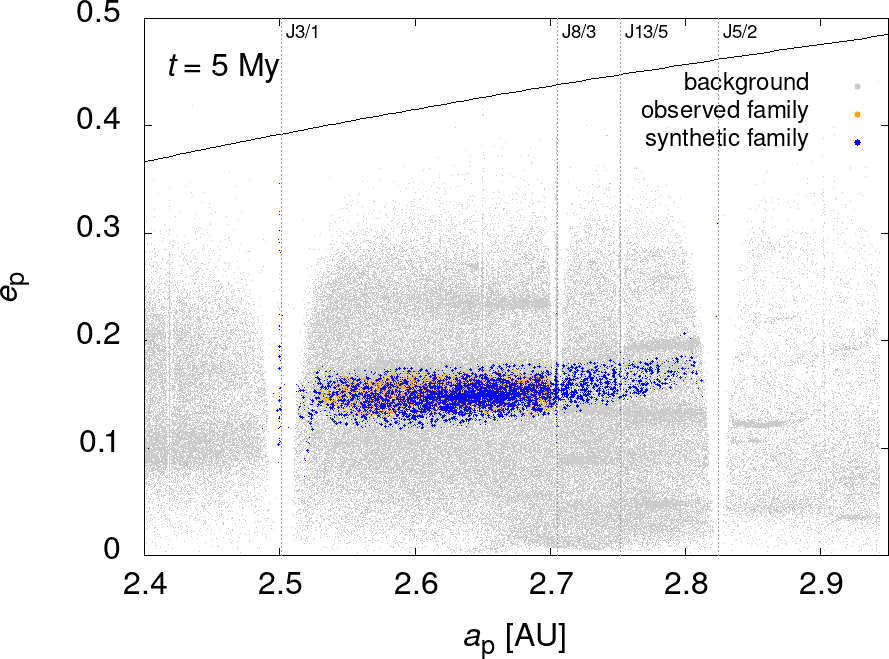
\includegraphics[width=0.49\textwidth]{obr/ae_5t.png}
	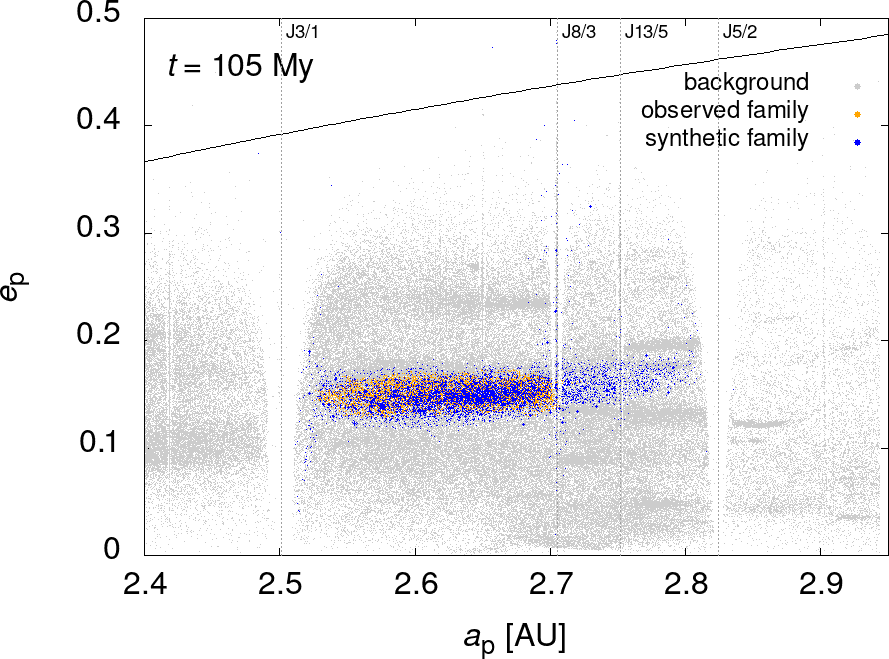
\includegraphics[width=0.49\textwidth]{obr/ae_105t.png}\\
	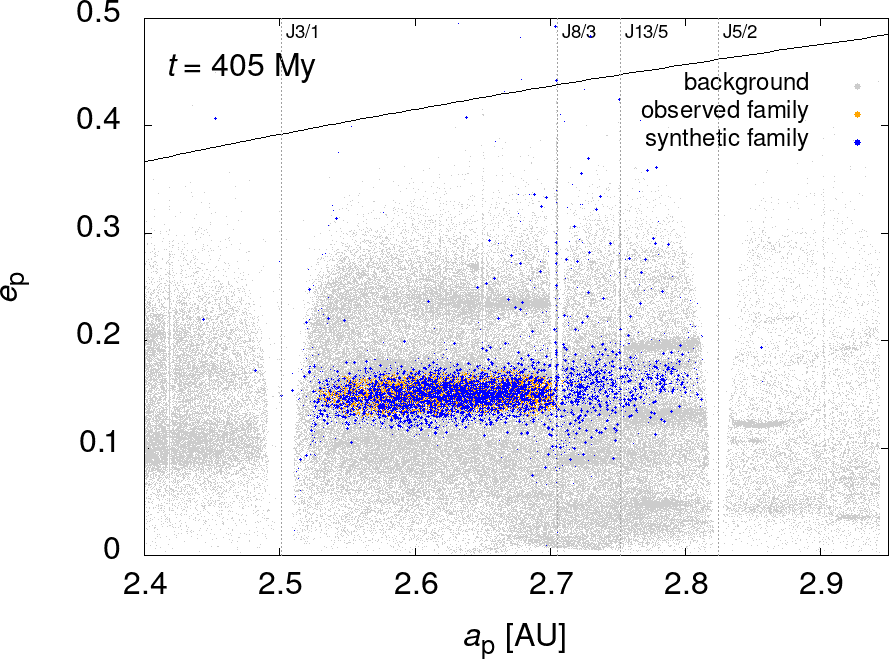
\includegraphics[width=0.49\textwidth]{obr/ae_405t.png}
	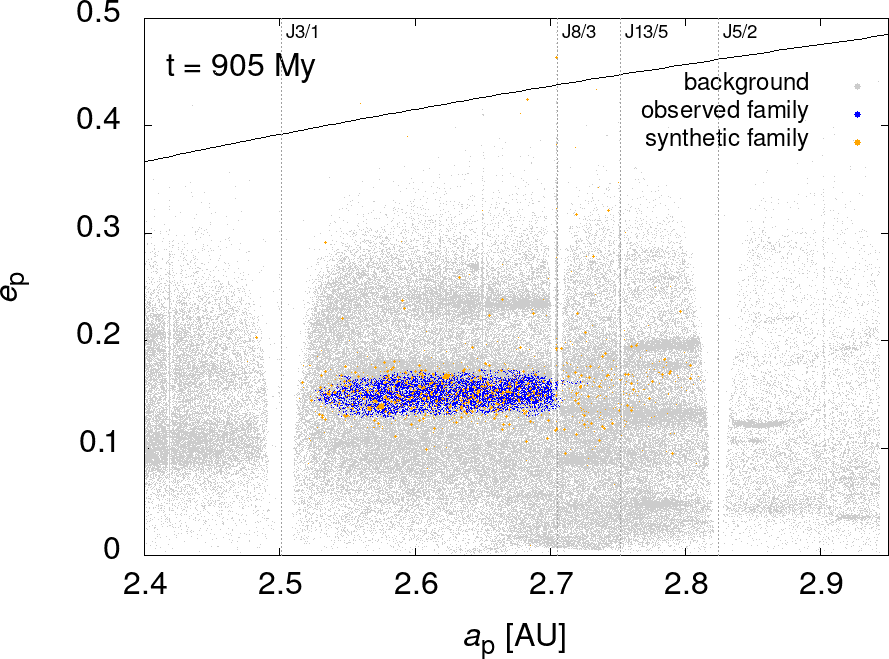
\includegraphics[width=0.49\textwidth]{obr/ae_905t.png}
	\caption{Výsledky simulace v prostoru $(a_{\rm p},\,e_{\rm p})$ v časech postupně $5$, $105$, $405$ a $905$ miliónů let. Fialové body označují simulovanou rodinu, modré tečky pozorovanou rodinu identifikovanou HCM a šedé pozadí a jiné okolní rodiny. Jsou také značeny nejvýznamější rezonance s Jupiterem J3/1, J8/3, J13/5 a J5/2. Černá křivka nahože označje hranici oblasti, kde je hlavní poloosa a excentricita tělesa taková, že dráha kříží dráhu Marsu. Podobná hranice existuje i pro Jupiter, ale ta se nachází mimo tyto grafy (přibližně kolem $e=0,65$). } \label{fig_ae_sim}
\end{figure}

Úvodní rozpad byl izotropní, ale kvůli specifickému výpočtu vlastních elementů dráhy z únikových rychlost pomocí Gaussových rovnic můžeme v čase $T=5\,{\rm My}$ pozorovat mírně nesymetrický tvar simulované rodiny. Dále si můžeme všimnout, že počáteční rodina je o něco větší než rodina pozorováná, což nám ale nevadí, protože vždy můžeme vybrat pouze podmnožinu planetek (neinteragují spolu). 

Lze pozorovat vliv rezonancí --- u těch nejsilnější (J3/1 a J5/2) se planetky nejvíce vychylují, když se nachází v oblasti tzv. separatrixy (šikmá hranice před a za rezonancí), načež se jejich excentricity začnou zvyšovat, čímž se dostanou do oblasti, kde kříží dráhy Marsu nebo Jupitera, což znamená, že se planetka dřív nebo později některé z těchto planet přiblíží a je prudce vychýlena ze své dráhy. U rezonance J3/1 lze vidět u některých těles naopak pokles excentricity, to ale může být znovu důsledek specifického výpočtu vlastní elementů dráhy (neexistuje žádný fyzikální význam). 

Kromě těchto dvou rezonancí lze také vidět vliv rezonancí vyšších řádů --- J8/3 a J13/5 jasně rozdělují planetky simulované rodiny do oblastí mezi rezonancemi, ze kterých planetky zřídkakdy přecházejí do jiné oblasti. Rezonance J8/3 je silnější, a proto se tělesa v její blízkosti v čase $T=105$ miliónů let rozšířila do pásu o velikosti $0,05<e_{\rm p}<0,5$, zatímco v blízkosti rezonance J13/5 pouze do pásu o velikosti $0,1<e_{\rm p}<0,23$.

V populaci pozadí lze také vidět velice slabé rezonance na $a\approx2,62\,{\rm AU}$ a $a\approx2,66\,{\rm AU}$ --- jejich působení na simulovanou rodinu nelze vidět na obrázcích v této práci, lze ale jejich velmi nepatrný vliv vidět při procházení všech obrázků z celé simulace.

Jednou z nezodpovězených otázek týkajících se této rodiny je, zda-li nepokračuje za rezonanci J5/2~\cite{nesvorny15}. Tento návrh můžeme ale i z této částečné simulace s jistotou vyvrátit, protože planetky rezonanci až na výjimky (viz obrázek ~\ref{fig:ae_sim} $t=405\,{\rm My}$) nepřeskakují, ale jsou jí vychylovány do oblastí křížení drah Marsu nebo Jupitera. 


\immediate\write18{convert -trim obr/ai_5.png obr/ai_5t.png}
\immediate\write18{convert -trim obr/ai_105.png obr/ai_105t.png}
\immediate\write18{convert -trim obr/ai_405.png obr/ai_405t.png}
\immediate\write18{convert -trim obr/ai_905.png obr/ai_905t.png}
\begin{figure}
	\centering
	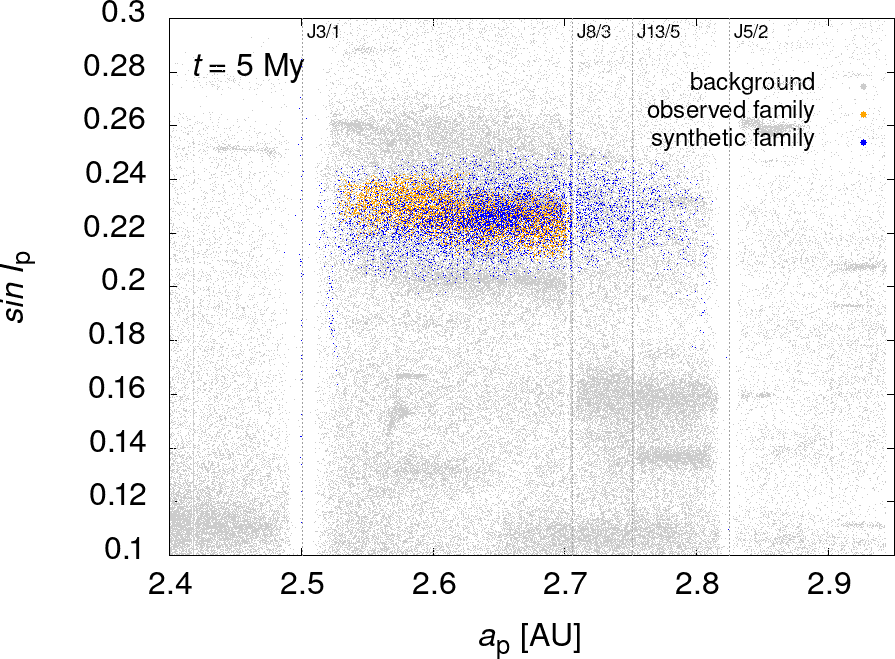
\includegraphics[width=0.49\textwidth]{obr/ai_5t.png}
	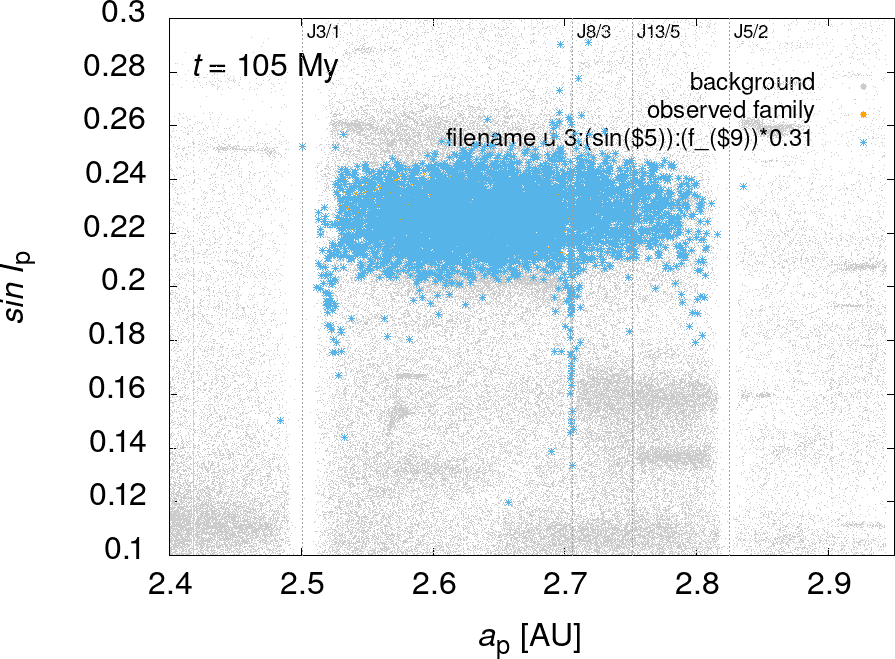
\includegraphics[width=0.49\textwidth]{obr/ai_105t.png}\\
	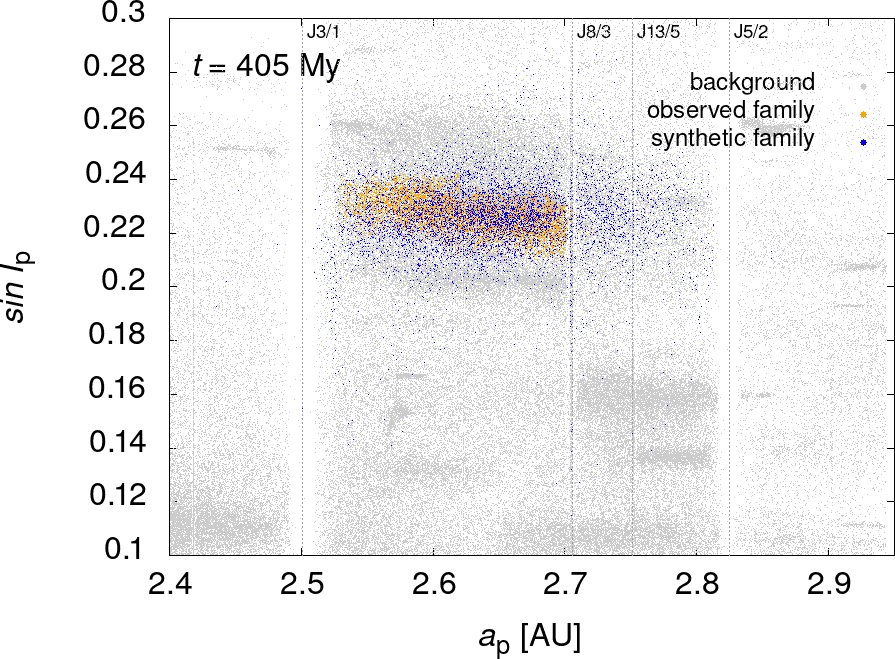
\includegraphics[width=0.49\textwidth]{obr/ai_405t.png}
	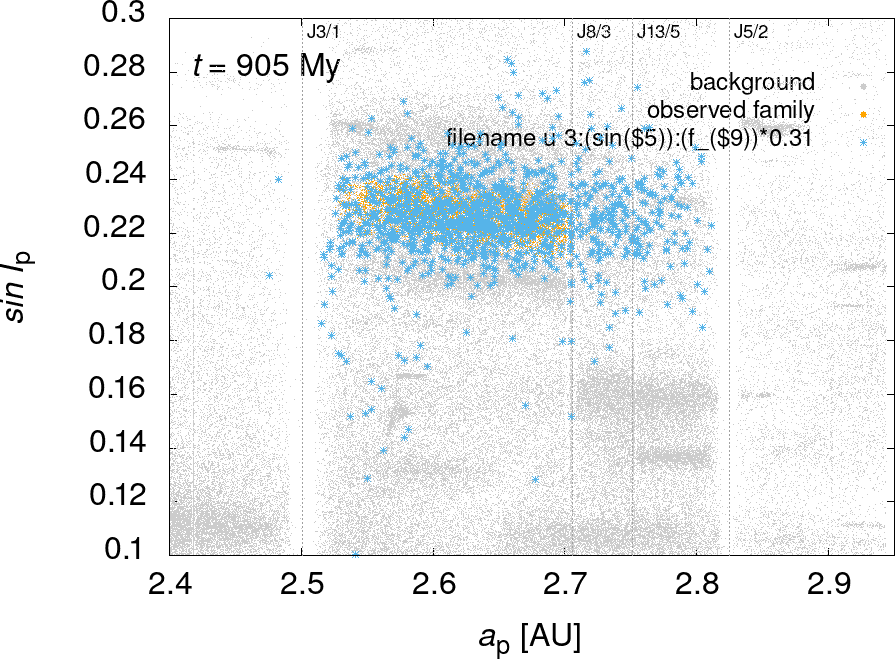
\includegraphics[width=0.49\textwidth]{obr/ai_905t.png}
	\caption{Výsledky simulace v prostoru $(a_{\rm p},\,\sin I_{\rm p})$ v časech postupně $5$, $105$, $405$ a $905$ miliónů let.} \label{fig:ai_sim}
\end{figure}

\immediate\write18{convert -trim obr/ei_5.png obr/ei_5t.png}
\immediate\write18{convert -trim obr/ei_105.png obr/ei_105t.png}
\immediate\write18{convert -trim obr/ei_405.png obr/ei_405t.png}
\immediate\write18{convert -trim obr/ei_905.png obr/ei_905t.png}
\begin{figure}
	\centering
	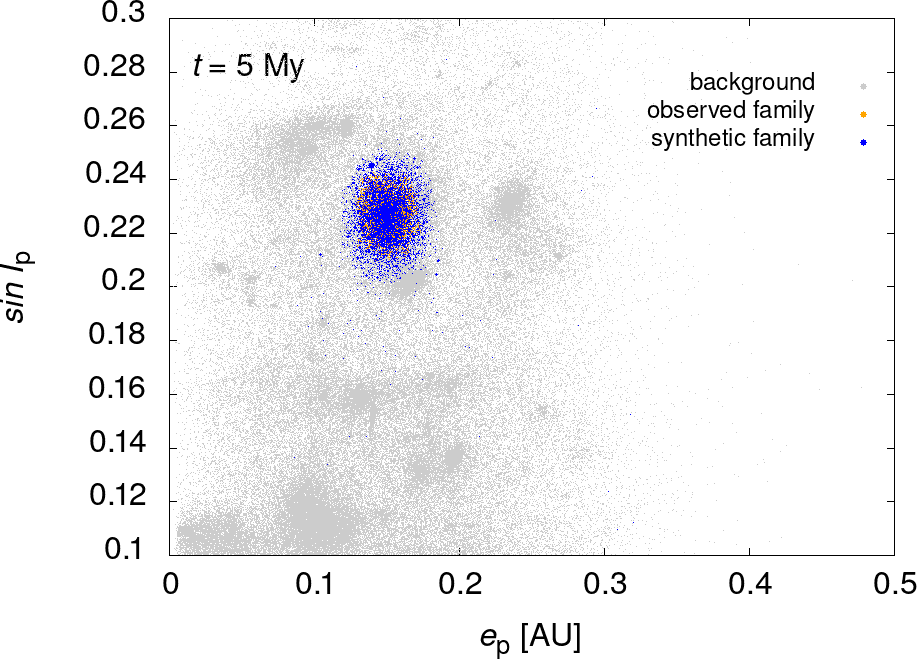
\includegraphics[width=0.49\textwidth]{obr/ei_5t.png}
	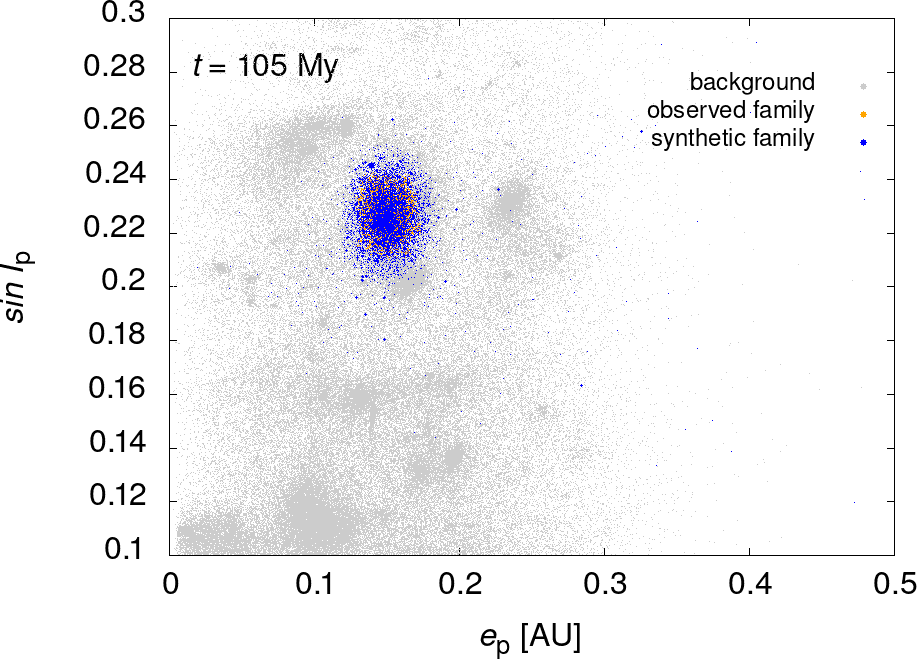
\includegraphics[width=0.49\textwidth]{obr/ei_105t.png}\\
	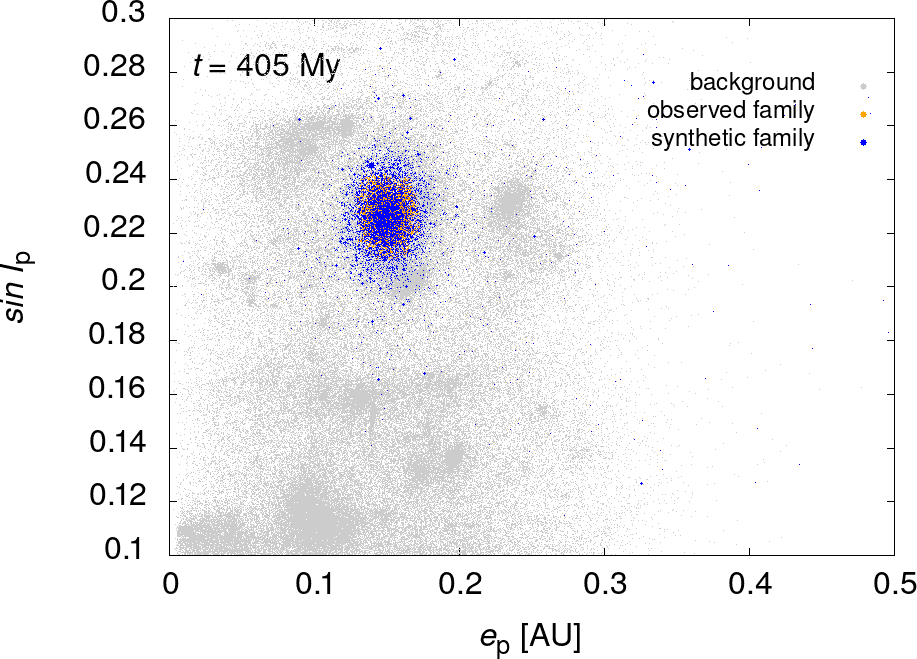
\includegraphics[width=0.49\textwidth]{obr/ei_405t.png}
	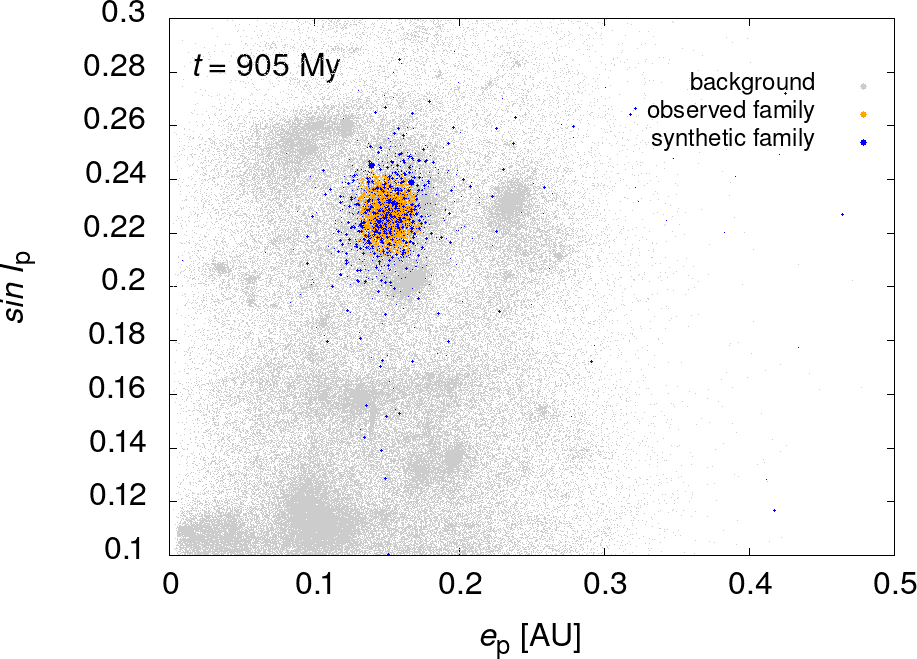
\includegraphics[width=0.49\textwidth]{obr/ei_905t.png}
	\caption{Výsledky simulace v prostoru $(e_{\rm p},\,i_{\rm p})$ v časech postupně $5$, $105$, $405$ a $905$ miliónů let.} \label{fig:ei_sim}
\end{figure}

\section{Odhad stáří}

K odhadu stáří rodiny použijeme statistickou metodu, popsanou v~\cite{broz11}, která funguje na principu rozdělení planetek jak pozorované, tak simulované rodiny do \uv{boxů} a následném porovnání počtů pozorovaných a simulovaných planetek v jednotlivých boxech.

Prvním krokem k provedení této metody je určení boxů. Protože se oblast mezi rezonancemi J8/3 a J13/5 zdá pro stáří rodiny významná, zvolili jsme boxy tak, aby se ve velké poloose mezi tyto rezonance vešly přesně tři. Dále jsme přidali $12$ boxů nalevo a $5$ napravo, to znamená, že spodní hranice celé oblasti je asi na $2,52\,{\rm AU}$ a horní asi na $2,81$


\chapter{Závěr}

%{{{ Bibliografie
\newpage

\printbibliography
%}}}
%{{{ Přílohy
\begin{appendices}
	\chapter{Ilustrace Eulerovy metody ve vektorové grafice v jazyce \I{Asymptote}} \label{app:asy}

	\begin{figure}[!htb]
	\centering
	\asyinclude{f_euler.asy}
	\end{figure}

	\lstinputlisting[language=Gnuplot]{asy/f_euler.asy}

	\chapter{Výpočet Keplerovy rovnice pomocí iterační metody} \label{app:kepit}
	Kód na výpočet Keplerovy rovnice, viz~\eqref{eq:kepler}, v programovacím jazyce Python pomocí iterační metody, jejímž předpisem je
	\begin{align*}
		E_{i+1}=M+e\sin{E_i}q\,, \quad \text{pro}\ i=0,\,1,\,2,\,\ldots
	\end{align*}
	kde bereme první odhad $E_0=M$. Algoritmus ukončíme, když dosáhneme přesnosti ${eps<10^{-13}}$, což odpovídá dvojité přesnosti reálných čísel v dnešních standardních programovacích jazycích.

	Tato metoda konverguje k řešení pouze pro excentricity $e<0,6627434\,$, pro vyšší excentricity je nutné využít jiné numerické metody.
\begin{lstlisting}[language=Python]
from math import sin

def kepler(M, e):
    """Solution of Kepler align"""
    eps = 1E-13
    E2 = M + e*sin(M)
    while True:
        E1 = E2
        E2 = M + e*sin(E1)
        if abs(E2 - E1) < eps:
            break 
    return E2
\end{lstlisting}
	\chapter{Výpočet polohy tělesa z~oskulačních elementů} \label{app:el2xyz}
	Kód na výpočet polohy tělesa $x,\,y,\,z$ z oskulačních elementů $a,\,e,\,i,\,\omega,\,\Omega,\,M$. Vstupním souborem je \I{bin.out}, což je výstupní soubor integrátoru SWIFT (nutno však nejprve použít program \I{follow2} na získání dat z binárního souboru $bin.dat$), který má formát prostého textu, kde jsou jednotlivé sloupce oddělené tabulátory. Výstup programu je ve formátu $t\,[{\rm Yr}]\ x\,[{\rm AU}]\ y\,[{\rm AU}]\ z\,[{\rm AU}]$ a lze ho použít pro vygenerování animace jako v~\ref{fig:trajec}.
	\begin{lstlisting}[language=Python]
from math import *

def el2xyz(path):
    """Conversion from orbital elements to xyz positions (from text file bin.out by program follow2)"""
    binout = open(path, 'r')
    for line in binout.readlines()
        l = line.split()
        id = int(l[0])
        if id > 0:
            t = float(l[1])
            a = float(l[2])
            e = float(l[3])
            inc = radians(float(l[4]))
            capom = radians(float(l[5]))
            omega = radians(float(l[6]))
            M = radians(float(l[7]))
    
            # Note: The approximation by 3 terms was not sufficient
            # E = M + (e-pow(e,3.0)/8.0)*sin(M) + pow(e,2)/2.0*sin(2.0*M) + pow(e,3)*3.0/8.0*sin(3.0*M)
            E = kepler(M, e)
            f = 2.0*atan(sqrt((1.0+e)/(1.0-e))*tan(E/2.0))
            r = a*(1-e*cos(E))
            x = r*(cos(capom)*cos(omega+f)-sin(capom)*sin(omega+f)*cos(inc))
            y = r*(sin(capom)*cos(omega+f)+cos(capom)*sin(omega+f)*cos(inc))
            z = r*sin(inc)*sin(omega+f)
            print (t + " " + str(x) + " " + str(y) + " " + str(z))

def main():
    if (len(sys.argv) >= 2):
        el2xyz(sys.argv[1])
    else:
        print "Usage el2xyz.py infile"

if __name__ == "__main__":
    main()
	\end{lstlisting}
\end{appendices}
%}}}
\end{document}
